% !TEX root = Tesi.tex
\chead{}
\chapter{Our approach to modeling}

After summarily describing three different streams of real usage data obtained both from the physical and the virtual world in the last chapter, we now focus on expanding those representations in a more detailed way with the help of the Model Driven Engineering techniques briefly described in \ref{model-driven-techniques}. 
Concretely, the first two section objectives are to illustrate the defining languages (metamodels) for both the real usage data and the eCommerce platform interactions used in the previous examples and generate actual models based upon them representing the very same information.
Finally, in the last section of this chapter, we will be using the very same generation for updating the previously instantiated models leveraging model transformation techniques based upon usage pattern detection resulting from the Big Data analysis.

\section{Real usage data modeling}

\subsection{Metamodel}

The representation of the real usage data starts from the definition of the metamodel which defines the languages and processes from which to form a model without making statements about its content. In fact, a metamodel is itself a model that is used to describe another model using a modeling language and at a different level of abstraction.  

The figure in \ref{fig:real-usage-data-metamodel-diagram} describes the processed metamodel as a UML Class Diagram accordingly to the data retrieved for our real usage data analysis.

\vspace{0.5cm}
\begin{figure}[H]
  \centering
    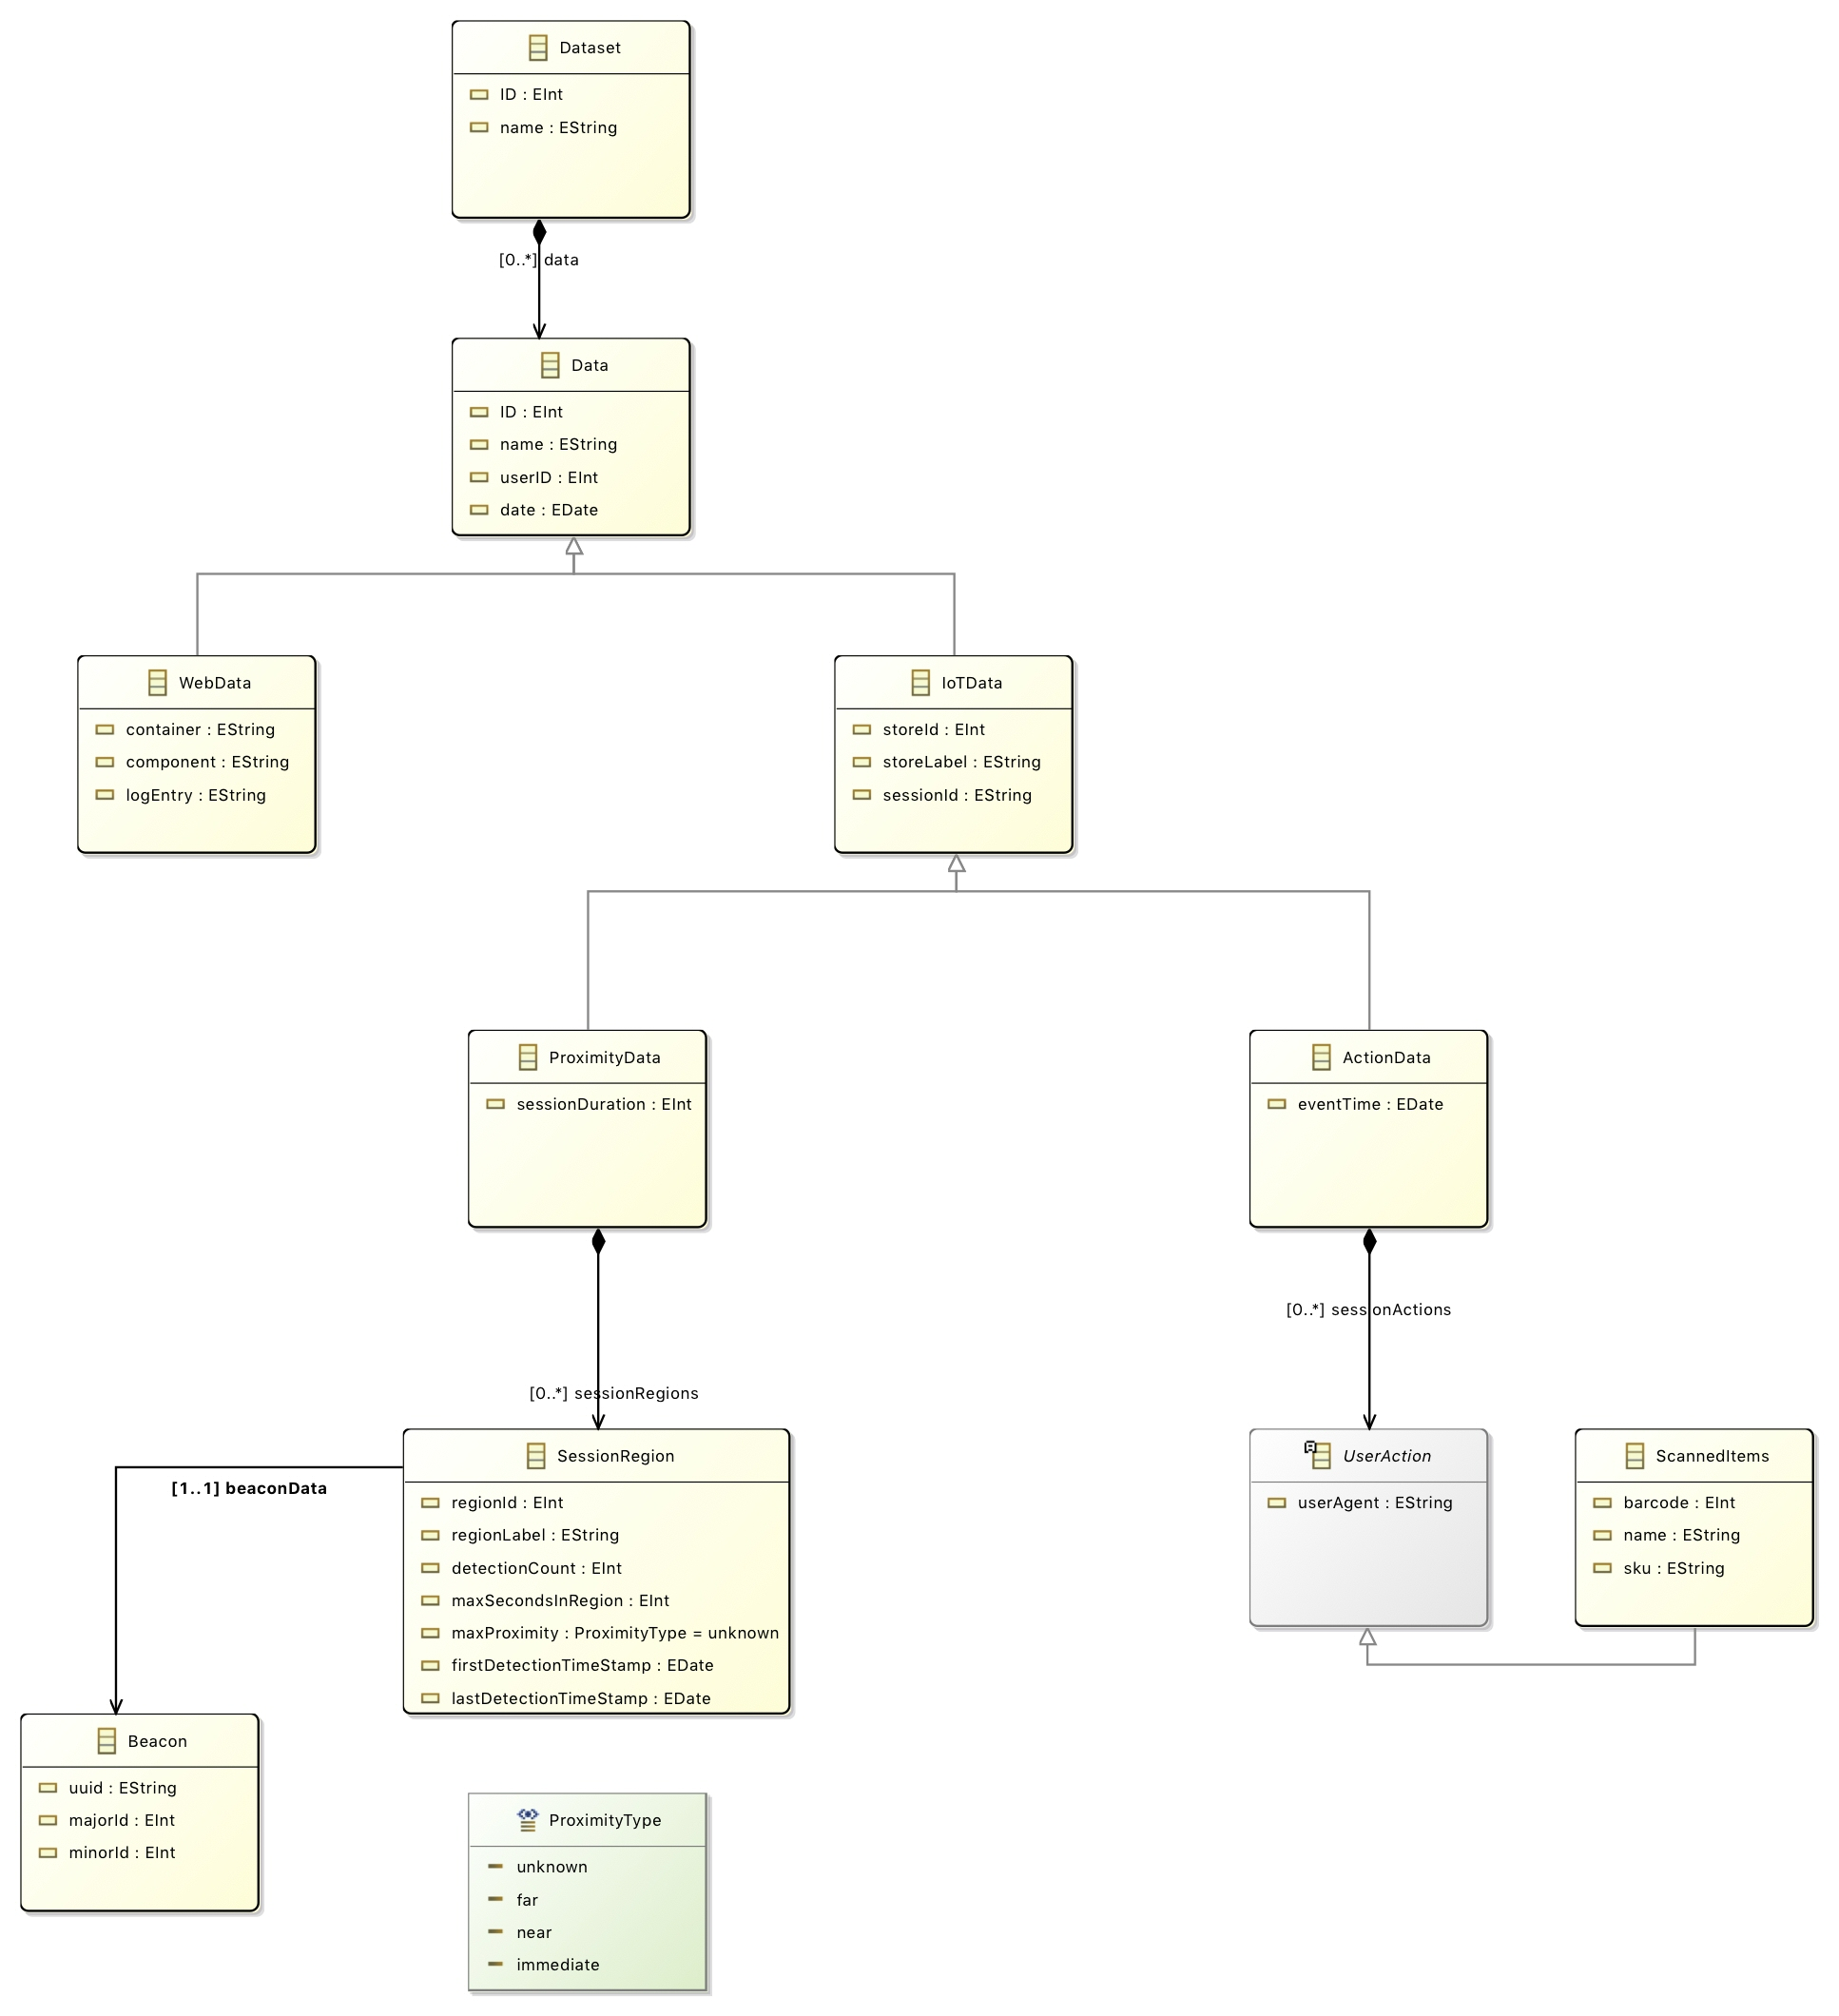
\includegraphics[height=19cm]{images/diagrams/RealUsageDataMetamodel.jpg}
  \caption{Real Usage Data Metamodel Diagram Class}
  \label{fig:real-usage-data-metamodel-diagram}
\end{figure}
\vspace{0.5cm}

\newpage
\subsection{Model}
\label{real-usage-data-model}
The RealUsageData metamodel defined above allow us to create dynamic instances which precisely map the real usage data collected from the web mining process and the IoT devices tracking. Figure \ref{fig:real-usage-data-model} illustrates this processed model in its eCore representation form in Eclipse and it is followed by the corrisponding XMI file content.

\vspace{0.5cm}
\begin{figure}[H]
  \centering
    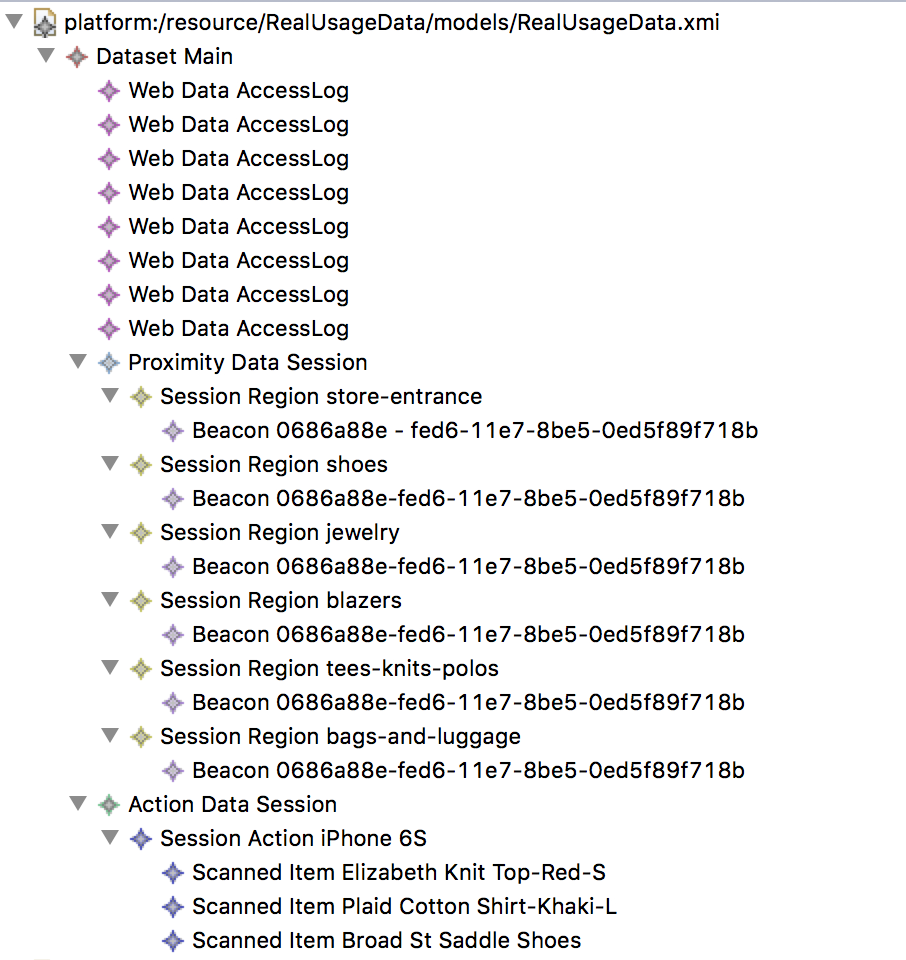
\includegraphics[height=12cm]{images/diagrams/RealUsageDataModel.png}
  \caption{Real Usage Data Model}
  \label{fig:real-usage-data-model}
\end{figure}
\vspace{0.5cm}

\lstset{language=XML}
\begin{lstlisting} 
<?xml version="1.0" encoding="UTF-8"?>
<RealUsageData:Dataset
    xmi:version="2.0"
    xmlns:xmi="http://www.omg.org/XMI"
    xmlns:xsi="http://www.w3.org/2001/XMLSchema-instance"
    xmlns:RealUsageData="RealUsageData"
    xsi:schemaLocation="RealUsageData ../metamodels/RealUsageData.ecore"
    ID="1" name="Main">
  <data xsi:type="RealUsageData:WebData"
      ID="1"
      name="AccessLog"
      userID="3045678"
      date="2017-11-29T17:06:49.000+0100"
      viewContainer="Homepage"
      viewComponent="TopMenu"
      eventType="click"
      parameterBindingGroup="Category/5"
      logEntry="GET /men.html / 200 0 - 29505"/>
  <data xsi:type="RealUsageData:WebData"
      ID="2"
      name="AccessLog"
      userID="3045678"
      date="2017-11-29T17:07:04.000+0100"
      viewContainer="Category #5"
      viewComponent="CategoryList"
      eventType="click"
      parameterBindingGroup="Category/15"
      logEntry="GET /men/shirts.html 200 0 - 29505"/>
  <data xsi:type="RealUsageData:WebData"
      ID="3"
      name="AccessLog"
      userID="3045678"
      date="2017-11-29T07:08:40.000+0100"
      viewContainer="Category #15"
      viewComponent="ProductList"
      eventType="click"
      parameterBindingGroup="Product/404"
      logEntry="GET /men/shirts/plaid-cotton-shirt-476.html 200 0 - 29505"/>
  <data xsi:type="RealUsageData:WebData"
      ID="4"
      name="AccessLog"
      userID="3045678"
      date="2017-12-04T06:37:15.000+0100"
      viewContainer="Product #404"
      viewComponent="RelatedProductList"
      eventType="click"
      parameterBindingGroup="Product/413"
      logEntry="GET /core-striped-sport-shirt-551.html 200 0 - 29505"/>
  <data xsi:type="RealUsageData:WebData"
      ID="5"
      name="AccessLog"
      userID="3045678"
      date="2017-12-04T06:37:21.000+0100"
      viewContainer=""
      viewComponent=""
      eventType="backButton"
      parameterBindingGroup=""
      logEntry="GET /men/shirts/plaid-cotton-shirt-476.html 200 0 - 29505"/>
  <data xsi:type="RealUsageData:WebData"
      ID="6"
      name="AccessLog"
      userID="3045678"
      date="2017-12-04T06:38:06.000+0100"
      viewContainer="Product #404"
      viewComponent="TopMenu"
      eventType="click"
      parameterBindingGroup="Category/16"
      logEntry="GET /men/tees-knits-and-polos.html 200 0 - 29505"/>
  <data xsi:type="RealUsageData:WebData"
      ID="7"
      name="AccessLog"
      userID="3045678"
      date="2017-12-04T06:38:20.000+0100"
      viewContainer="Category #16"
      viewComponent="TopSearch"
      eventType="submit"
      parameterBindingGroup="SearchText/blazer"
      logEntry="GET /catalogsearch/result/?q=blazer 200 0 - 29505"/>
  <data xsi:type="RealUsageData:WebData"
      ID="8"
      name="AccessLog"
      userID="3045678"
      date="2017-12-04T06:38:20.000+0100"
      viewContainer="Search Results"
      viewComponent="ProductList"
      eventType="click"
      parameterBindingGroup="Product/407"
      logEntry="GET /stretch-cotton-blazer-587.html 200 0 - 29505"/>
  <data xsi:type="RealUsageData:ProximityData"
      ID="9"
      name="Session"
      userID="3045678"
      date="2018-02-21T18:16:07.000+0100"
      storeId="8784"
      storeLabel="Madison1"
      sessionId="89376f84-065b -11e8- ba89-0ed5f89f718b"
      sessionDuration="345">
    <sessionRegions
        regionId="156"
        regionLabel="store-entrance"
        detectionCount="2"
        maxSecondsInRegion="5"
        firstDetectionTimeStamp="2018-02-21T18:09:07.000+0100"
        lastDetectionTimeStamp="2018-02-21T18:16:02.000+0100">
      <beaconData
          uuid="0686a88e - fed6-11e7-8be5-0ed5f89f718b"
          majorId="2553"
          minorId="79"/>
    </sessionRegions>
    <sessionRegions
        regionId="645"
        regionLabel="shoes"
        detectionCount="1"
        maxSecondsInRegion="24"
        maxProximity="near"
        firstDetectionTimeStamp="2018-02-21T18:09:20.000+0100"
        lastDetectionTimeStamp="2018-02-21T18:09:20.000+0100">
      <beaconData
          uuid="0686a88e-fed6-11e7-8be5-0ed5f89f718b"
          majorId="19029"
          minorId="49"/>
    </sessionRegions>
    <sessionRegions
        regionId="6875"
        regionLabel="jewelry"
        detectionCount="1"
        maxSecondsInRegion="15"
        maxProximity="far"
        firstDetectionTimeStamp="2018-02-21T18:10:15.000+0100"
        lastDetectionTimeStamp="2018-02-21T18:10:15.000+0100">
      <beaconData
          uuid="0686a88e-fed6-11e7-8be5-0ed5f89f718b"
          majorId="38415"
          minorId="59"/>
    </sessionRegions>
    <sessionRegions
        regionId="2563"
        regionLabel="blazers"
        detectionCount="1"
        maxSecondsInRegion="195"
        maxProximity="immediate"
        firstDetectionTimeStamp="2018-02-21T18:11:01.000+0100"
        lastDetectionTimeStamp="2018-02-21T18:11:01.000+0100">
      <beaconData
          uuid="0686a88e-fed6-11e7-8be5-0ed5f89f718b"
          majorId="25911"
          minorId="27"/>
    </sessionRegions>
    <sessionRegions
        regionId="456"
        regionLabel="tees-knits-polos"
        detectionCount="1"
        maxSecondsInRegion="10"
        maxProximity="immediate"
        firstDetectionTimeStamp="2018-02-21T18:14:56.000+0100"
        lastDetectionTimeStamp="2018-02-21T18:14:56.000+0100">
      <beaconData
          uuid="0686a88e-fed6-11e7-8be5-0ed5f89f718b"
          majorId="42037"
          minorId="36"/>
    </sessionRegions>
    <sessionRegions
        regionId="998"
        regionLabel="bags-and-luggage"
        detectionCount="1"
        maxSecondsInRegion="7"
        maxProximity="far"
        firstDetectionTimeStamp="2018-02-21T18:15:12.000+0100"
        lastDetectionTimeStamp="2018-02-21T18:15:12.000+0100">
      <beaconData
          uuid="0686a88e-fed6-11e7-8be5-0ed5f89f718b"
          majorId="37931"
          minorId="85"/>
    </sessionRegions>
  </data>
  <data xsi:type="RealUsageData:ActionData"
      ID="10"
      name="Session"
      userID="3045678"
      date="2018-02-22T15:27:09.000+0100"
      storeId="8784"
      storeLabel="Madison1"
      sessionId="89376f84-065b-11e8-ba89-0ed5f89f718b"
      sessionDuration="456">
    <sessionActions
        userAgent="iPhone 6S">
      <scannedItems
          barcode="042100005264"
          name="Elizabeth Knit Top-Red-S"
          sku="wbk012c-Red-S"/>
      <scannedItems
          barcode="042100005931"
          name="Plaid Cotton Shirt-Khaki-L"
          sku="msj006c-Khaki-L"/>
      <scannedItems
          barcode="042100007717"
          name="Broad St Saddle Shoes"
          sku="shm00110"/>
    </sessionActions>
  </data>
</RealUsageData:Dataset>
\end{lstlisting}
\vspace{0.5cm}
\section{eCommerce application modeling}

As per briefly introduced in \ref{the-ifml-language}, IFML is used to design platform independent-level models which can be used to define the interactions between the users of an application and the application itself. 
At its core, IFML is meant to be flexible and straightforward, but perhaps more importantly, the language is intended to be abstract to provide the possibility of defining the main traits of an application front end making as few visual commitments as possible. Furthermore, its extendibility  allows modelers and designers to specialize specific components enriching the semantics of their models and making the diagrams more readable.

In fact, the models generated using IFML describe the user interface components required at the front-end of the application, without specifying layout details of these elements enhancing the separation of concerns among developers and UX designers where the latter build the user interface accordingly to an interaction flow model. Besides defining components of the User Interface, these models explain how data flows among different sections of the application upon triggering events and introduces the business logic carried out using this data.

\subsection{IFML Metamodel}

The IFML metamodel is organized into three packages: the Core package, the Extension package and the DataTypes package. The Core package contains the concepts that build up the interaction infrastructure of the language concerning InteractionFlowElements, InteractionFlows and Parameters. The Extension package extends the Core package components with more complex behaviors. The DataTypes package contains the custom data types defined by IFML.

\vspace{0.5cm}
\begin{figure}[H]
  \centering
    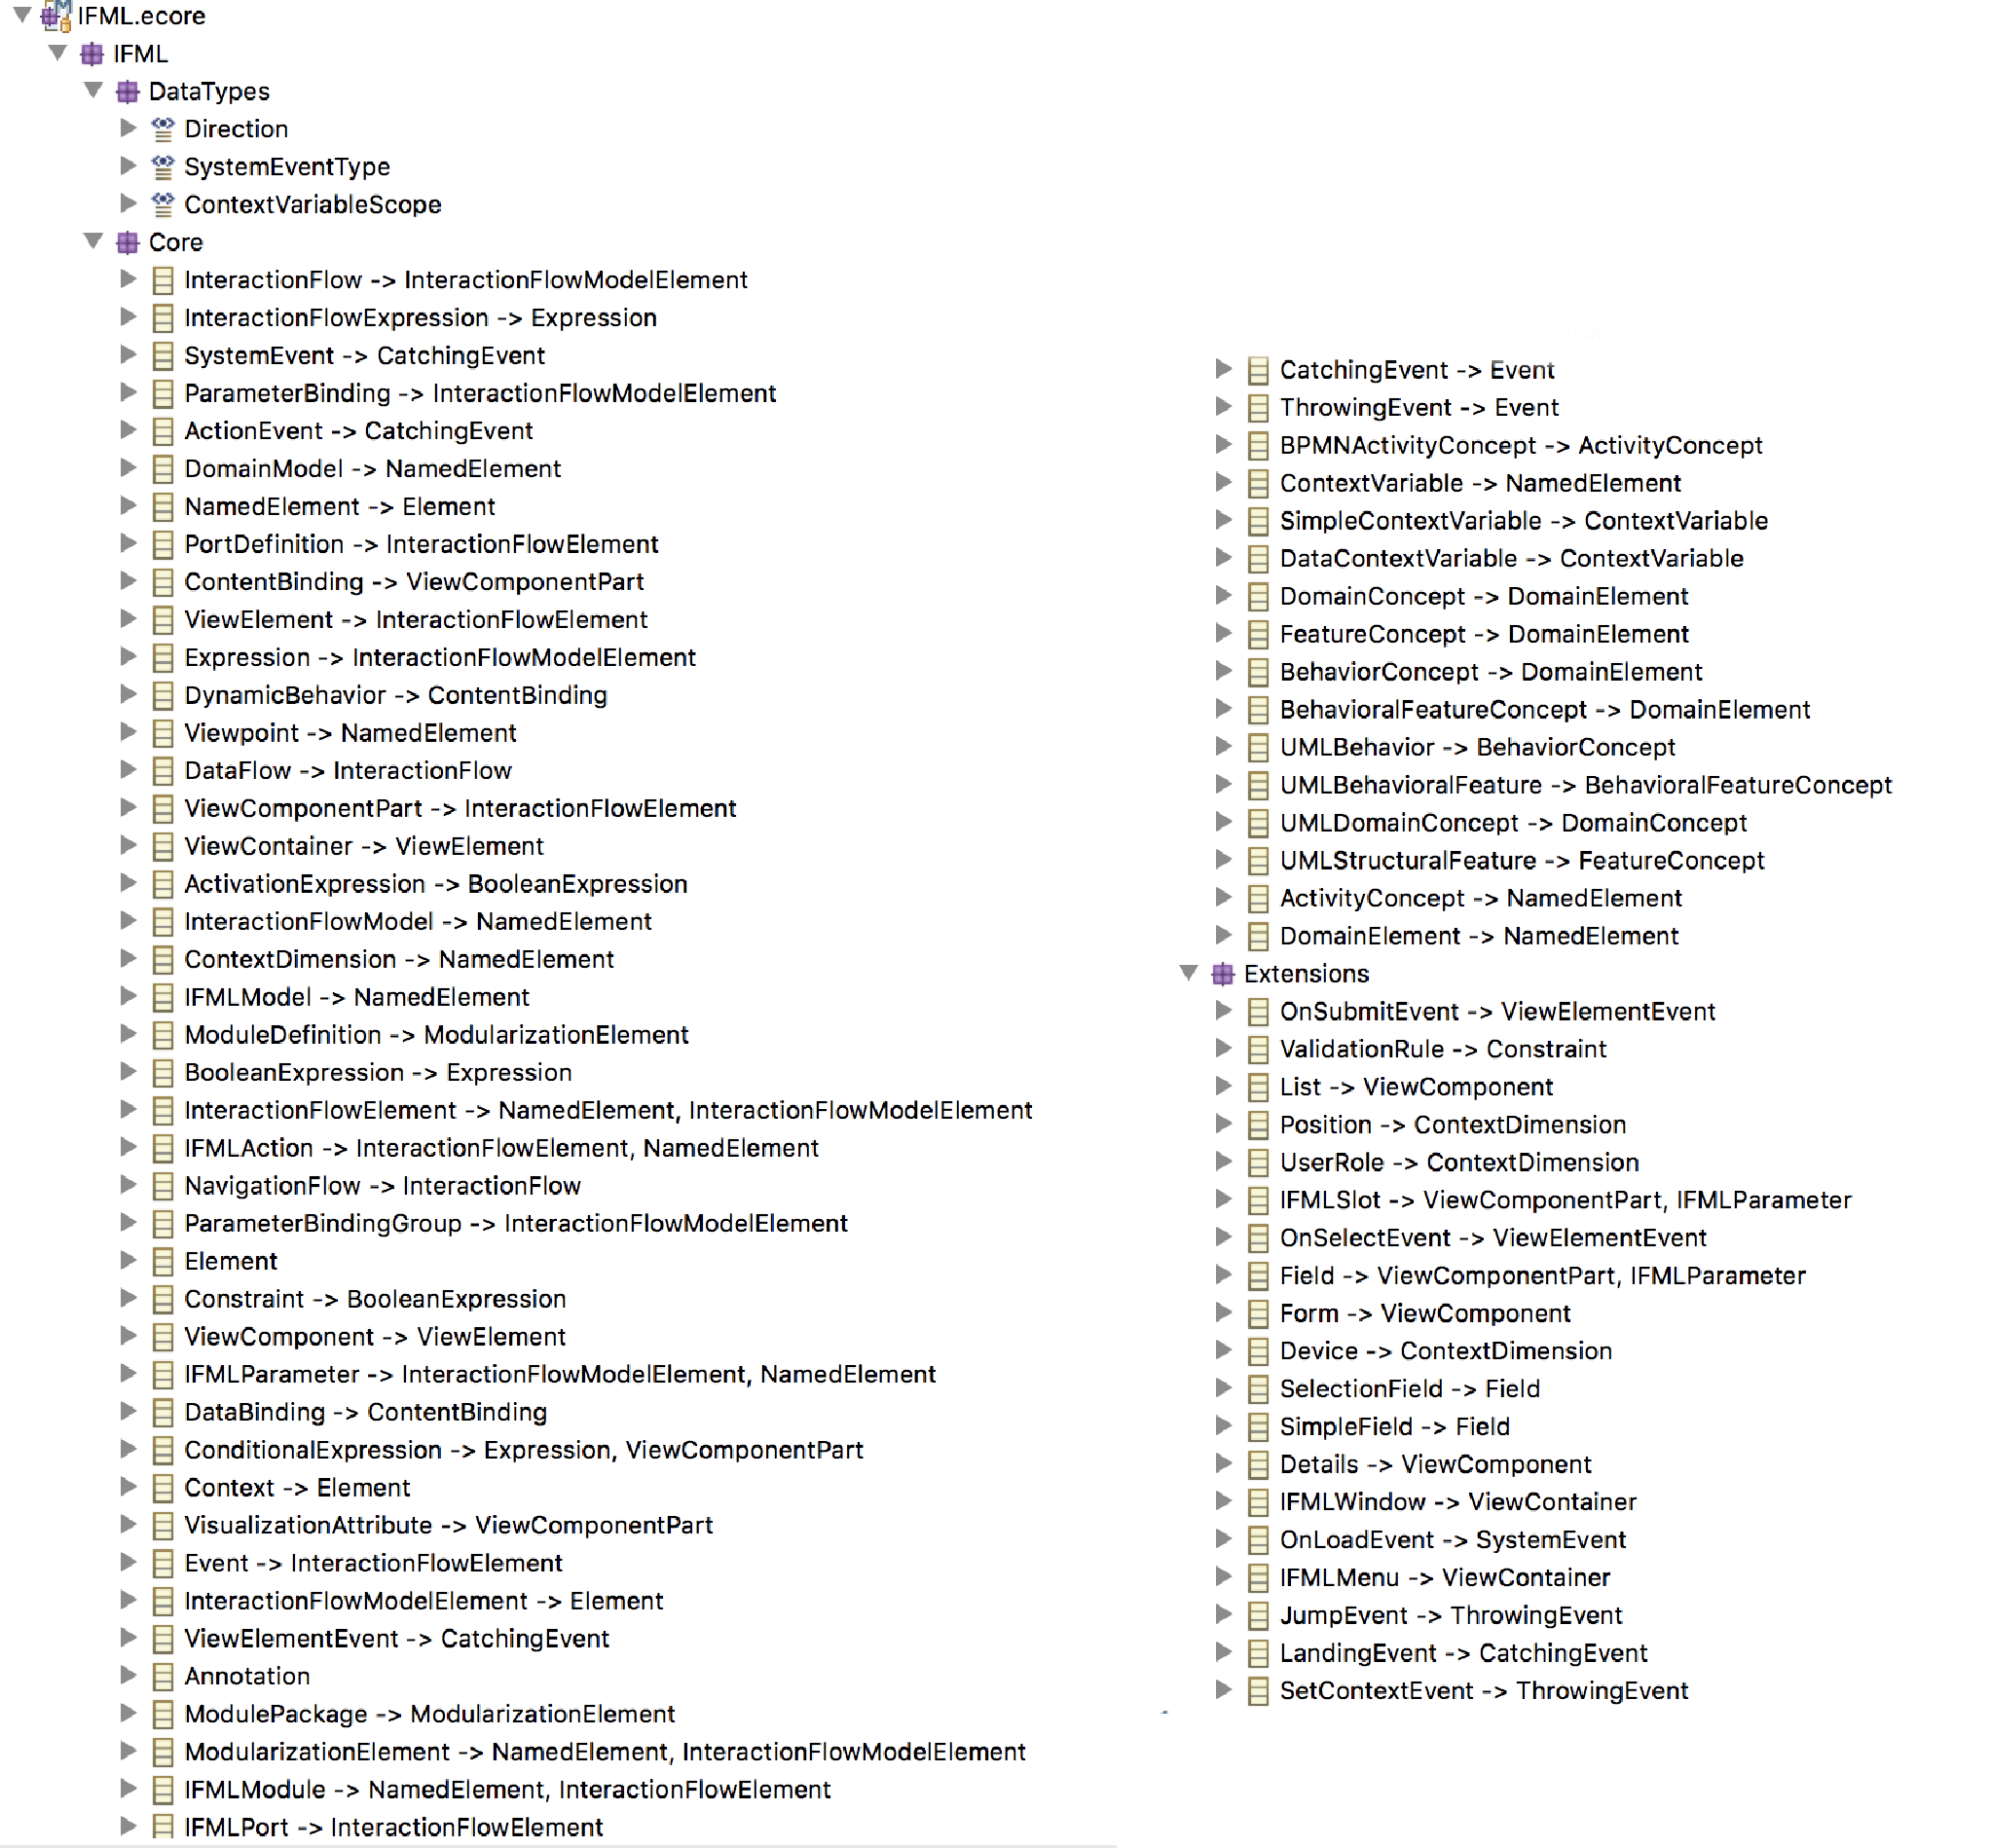
\includegraphics[width=14cm]{images/diagrams/ifml-ecore.png}
  \caption{IFML eCore representation}
  \label{fig:ifml-ecore-representation}
\end{figure}
\vspace{0.5cm}

By using the primitive data types from the UML metamodel and a UML representation for the IFML Domain Model, the IFML metamodel specifies a set of UML metaclasses as the foundation for the IFML metaclasses.

The following is the structure of the high-level representation of the IFML metamodel and its areas of concern:

\begin{itemize}
  \item IFML Model
  \item Interaction Flow Model
  \item Interaction Flow Elements
  \item View Elements
  \item Events
  \item Specific Events and View Components
  \item Parameters
  \item Expressions
  \item ContentBinding
\end{itemize}

Figure \ref{fig:simple-ifml-core-model} shows an excerpt of the IFML metamodel. As can be seen, IFMLModel is the top-level container of all the model elements and represents an IFML model. It contains an InteractionFlowModel which is the user view of an application, a DomainModel represented in UML and optionally ViewPoints. The concepts extending ViewContainer, ViewComponets, ViewComponentPart, and ViewElementEvent represent the visual elements of an IFML model.

\vspace{0.5cm}
\begin{figure}[H]
  \centering
    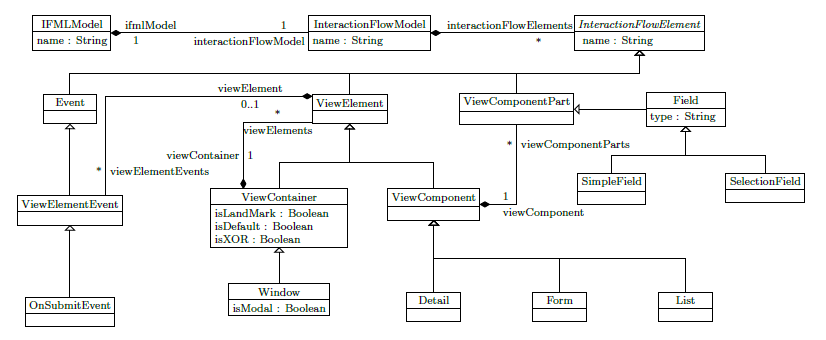
\includegraphics[width=12cm]{images/diagrams/ifml-metamodel.png}
  \caption{Simple eCore model of an IFML subset.}
  \label{fig:simple-ifml-core-model}
\end{figure}
\vspace{0.5cm}

\subsection{Model}

As per mentioned in the last subsection, interaction flow models are described using the Interaction Flow Modelling Language and, together with the domain model and optionally viewpoints, they form the core of the IFML model.

Essentially, the domain model objective is offering to the interaction flow references about the content available. An example of a domain model for an e-commerce website is given in Figure \ref{fig:domain-model-uml-ecommerce}   

\vspace{0.5cm}
\begin{figure}[H]
  \centering
    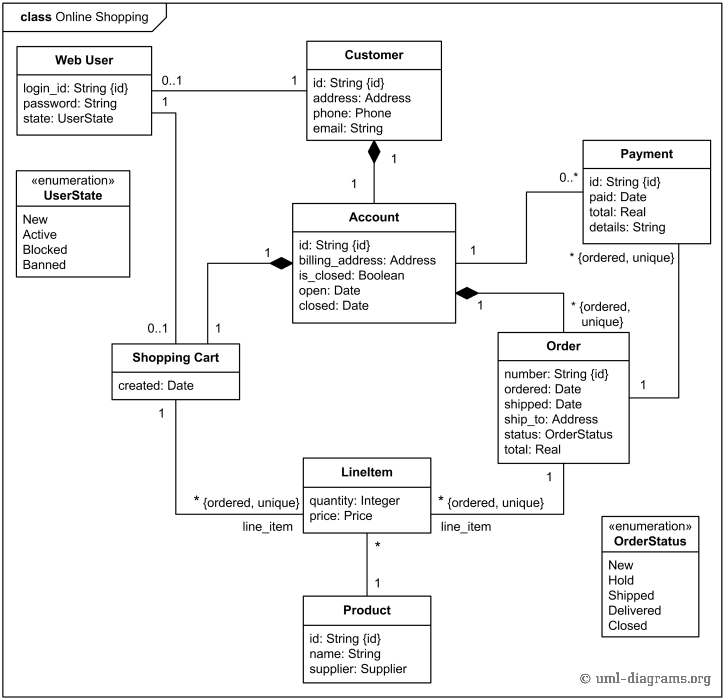
\includegraphics[width=12cm]{images/diagrams/domain-model-uml-ecommerce.png}
  \caption{Domain Model UML Class Diagram ecommerce example.}
  \label{fig:domain-model-uml-ecommerce}
\end{figure}
\vspace{0.5cm}

Although some partial IFML model representations for the Madison Island eCommerce platform have been already summarily introduced in \ref{navigational-modeling-for-the-web}, in this subsection we examine the most important ones in more detail and with a more global approach not strictly related to the navigational modeling. The final goal is to model, taking advantage of the IFML metamodel described just above, an IFML model which would represent the main pages and website interactions.

\subsubsection{Global overview}

The Madison Island Interaction Model is formed by a different combination of \textit{IFMLWindow} elements connected through \textit{IFMLAction}s reacting to distinct \textit{Events} with different \textit{ParameterBindings}. The detail of the modeling is contextual to the purpose of this thesis work; consequently, not all the possible interactions and elements presented on the website have been added to the IFMLModel in order to keep the model design lightweight and reduce its complexity. Overall, the principal \textit{IFMLWindow} standalone nodes have been described with more detail compared to others shared \textit{ViewContainer} elements, such as the Header and the Footer. In Figure \ref{fig:ifml-before-global} a visual representation of the IFMLDiagram corresponding to the main \textit{IFMLModel} for the Madison Island eCommerce platform is presented.

\begin{figure}[H]
  \centering
    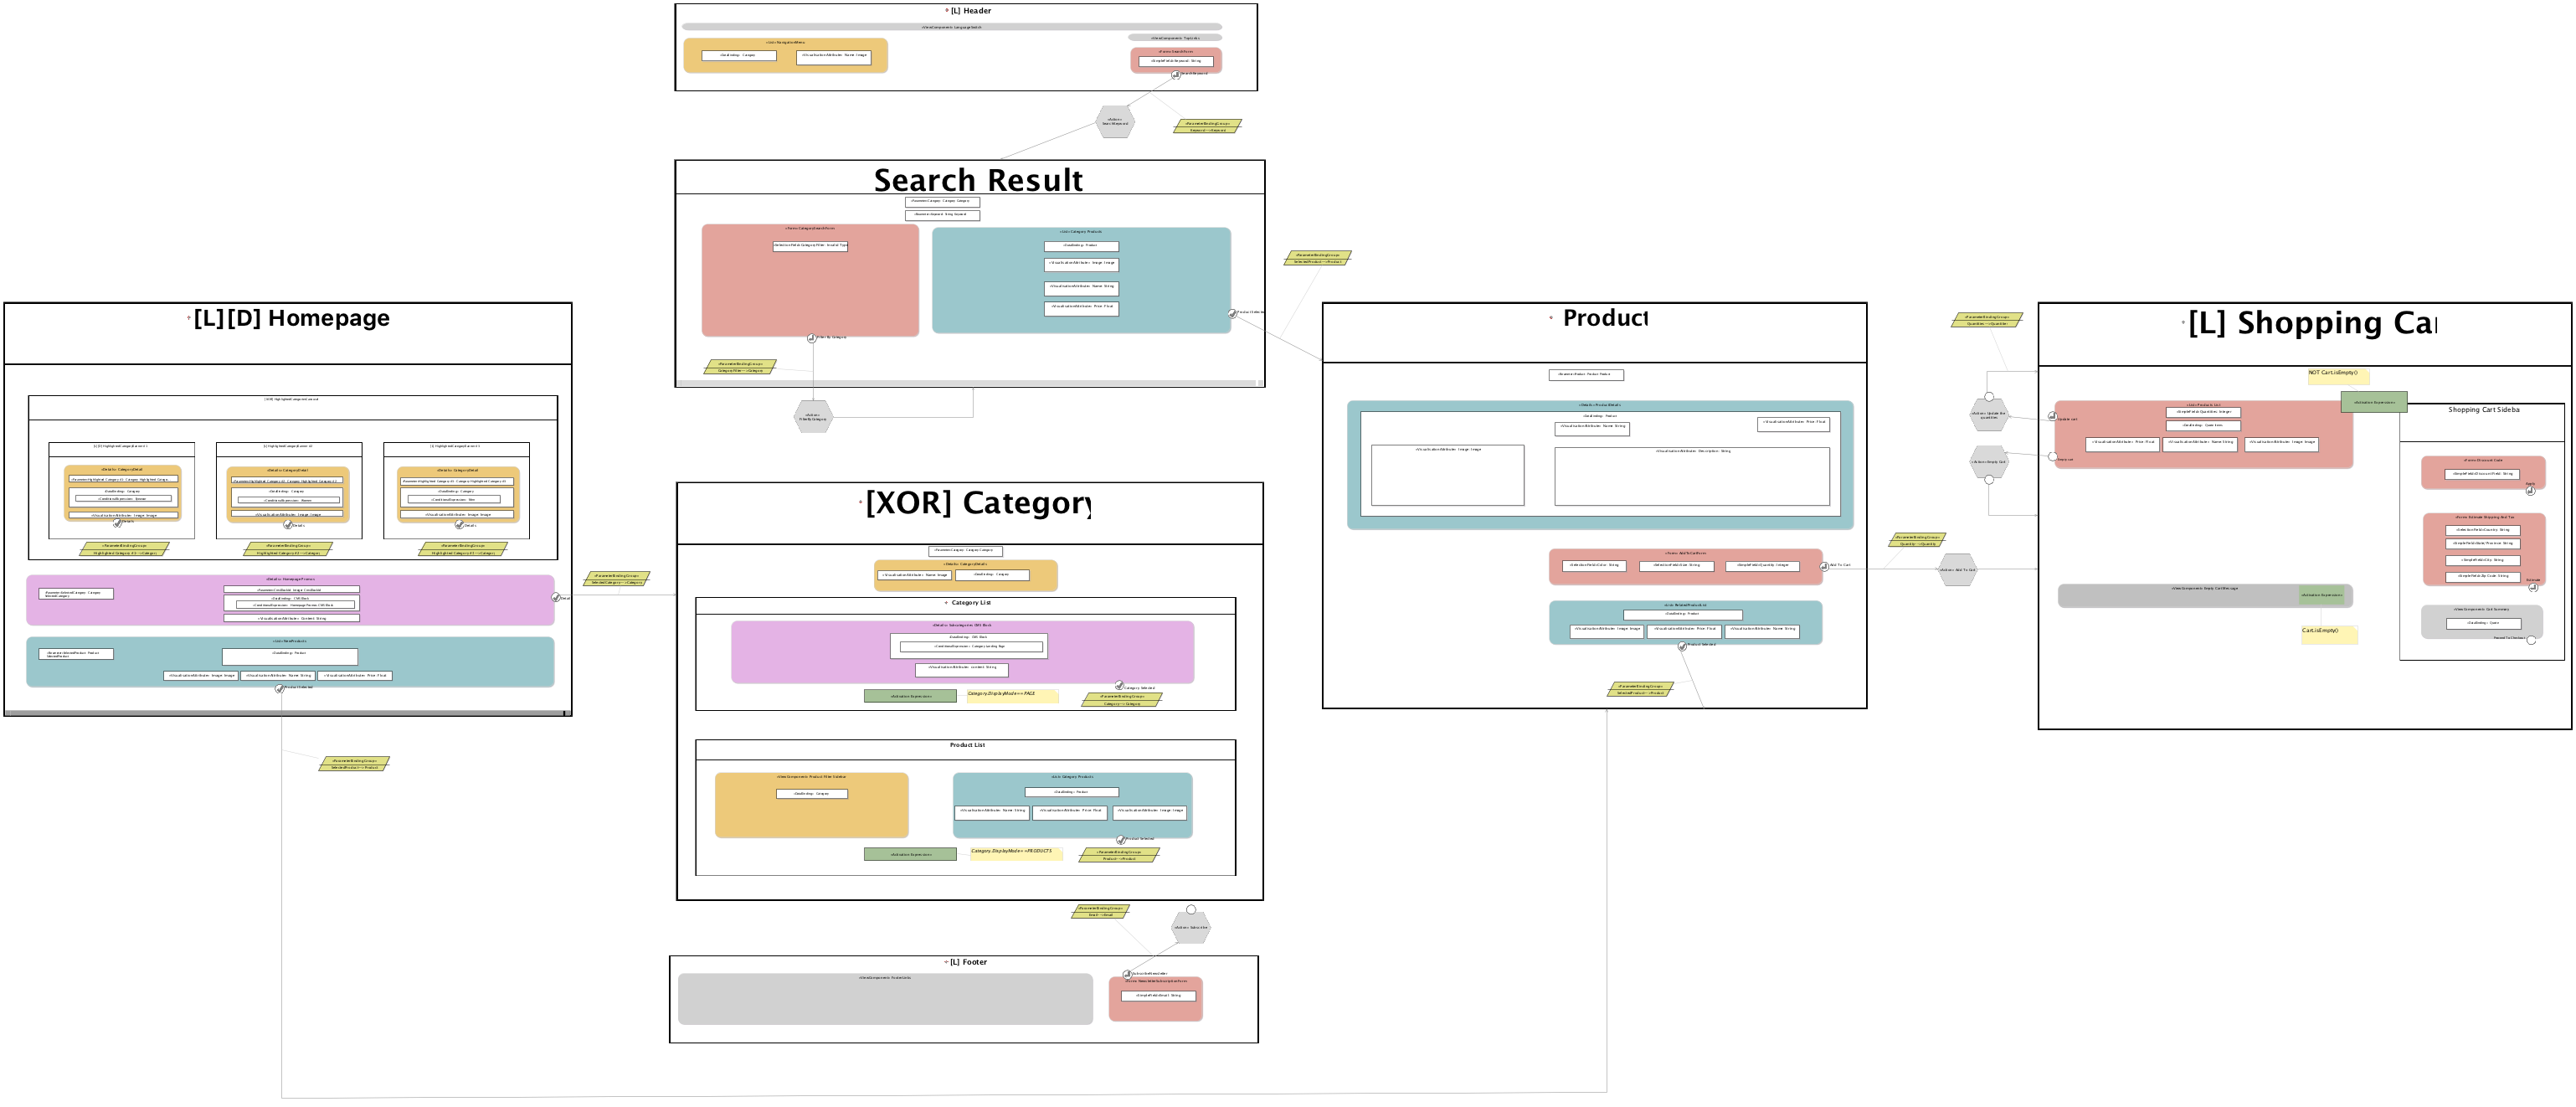
\includegraphics[height=10cm,angle=-90] {images/diagrams/before/ifml-global.png}
  \caption{Main Madison Island IFML Diagram}
  \label{fig:ifml-before-global}
\end{figure}

\subsubsection{Homepage overview}

The Madison Island Interaction Model for the Homepage (Figure \ref{fig:desktop-before-homepage} and \ref{fig:ifml-before-homepage}) is composed by a parent \textit{IFMLWindow} element which contains three children elements: respectively another \textit{IFMLWindow} for the Highlighted Categories Carousel, a \textit{Detail View Component} for the Homepage promos CMS Block and a \textit{List View Component} for the New Products sections bound to the Product Entity of the domain model. The HighlightedCategoriesCarousel Window is in \textit{XOR mode} representing three possible scenarios for the category to promote with the highest priority within the carousel mechanism. Each data binding within all these view containers is limited by a \textit{Conditional Expressions} defining the instance of the content to show.

\vspace{0.5cm}
\begin{figure}[H]
  \centering
    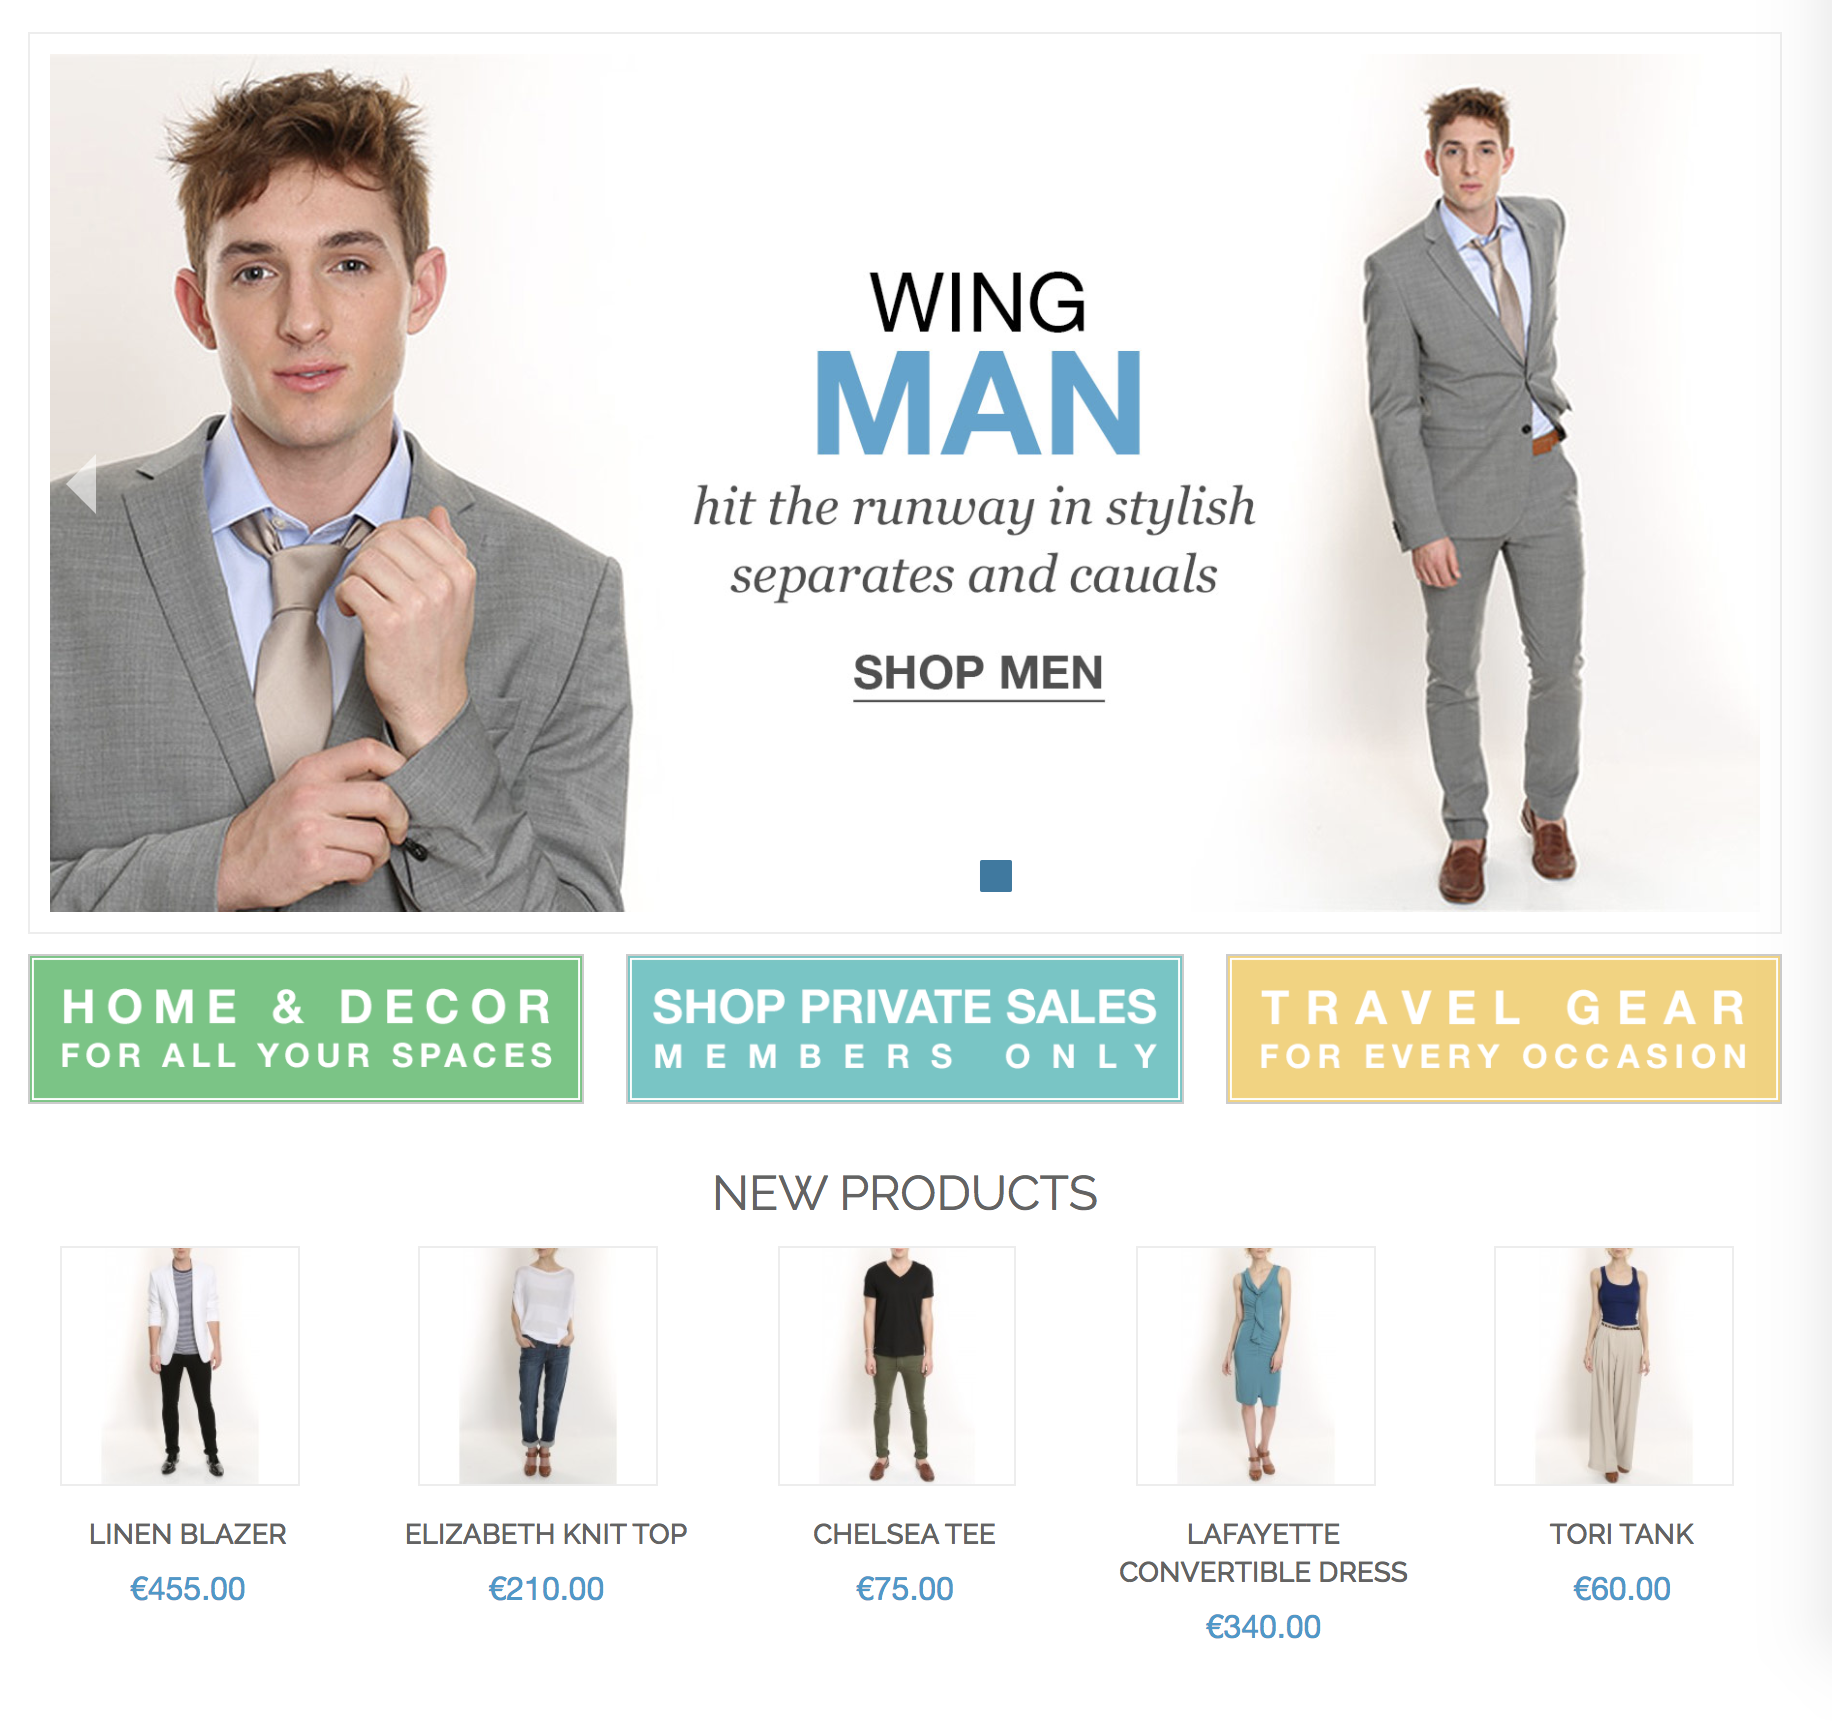
\includegraphics[height=7cm]{images/diagrams/before/desktop-homepage.png}
  \caption{Homepage Desktop Version}
  \label{fig:desktop-before-homepage}
\end{figure}
\vspace{0.5cm}

\begin{figure}[H]
  \centering
    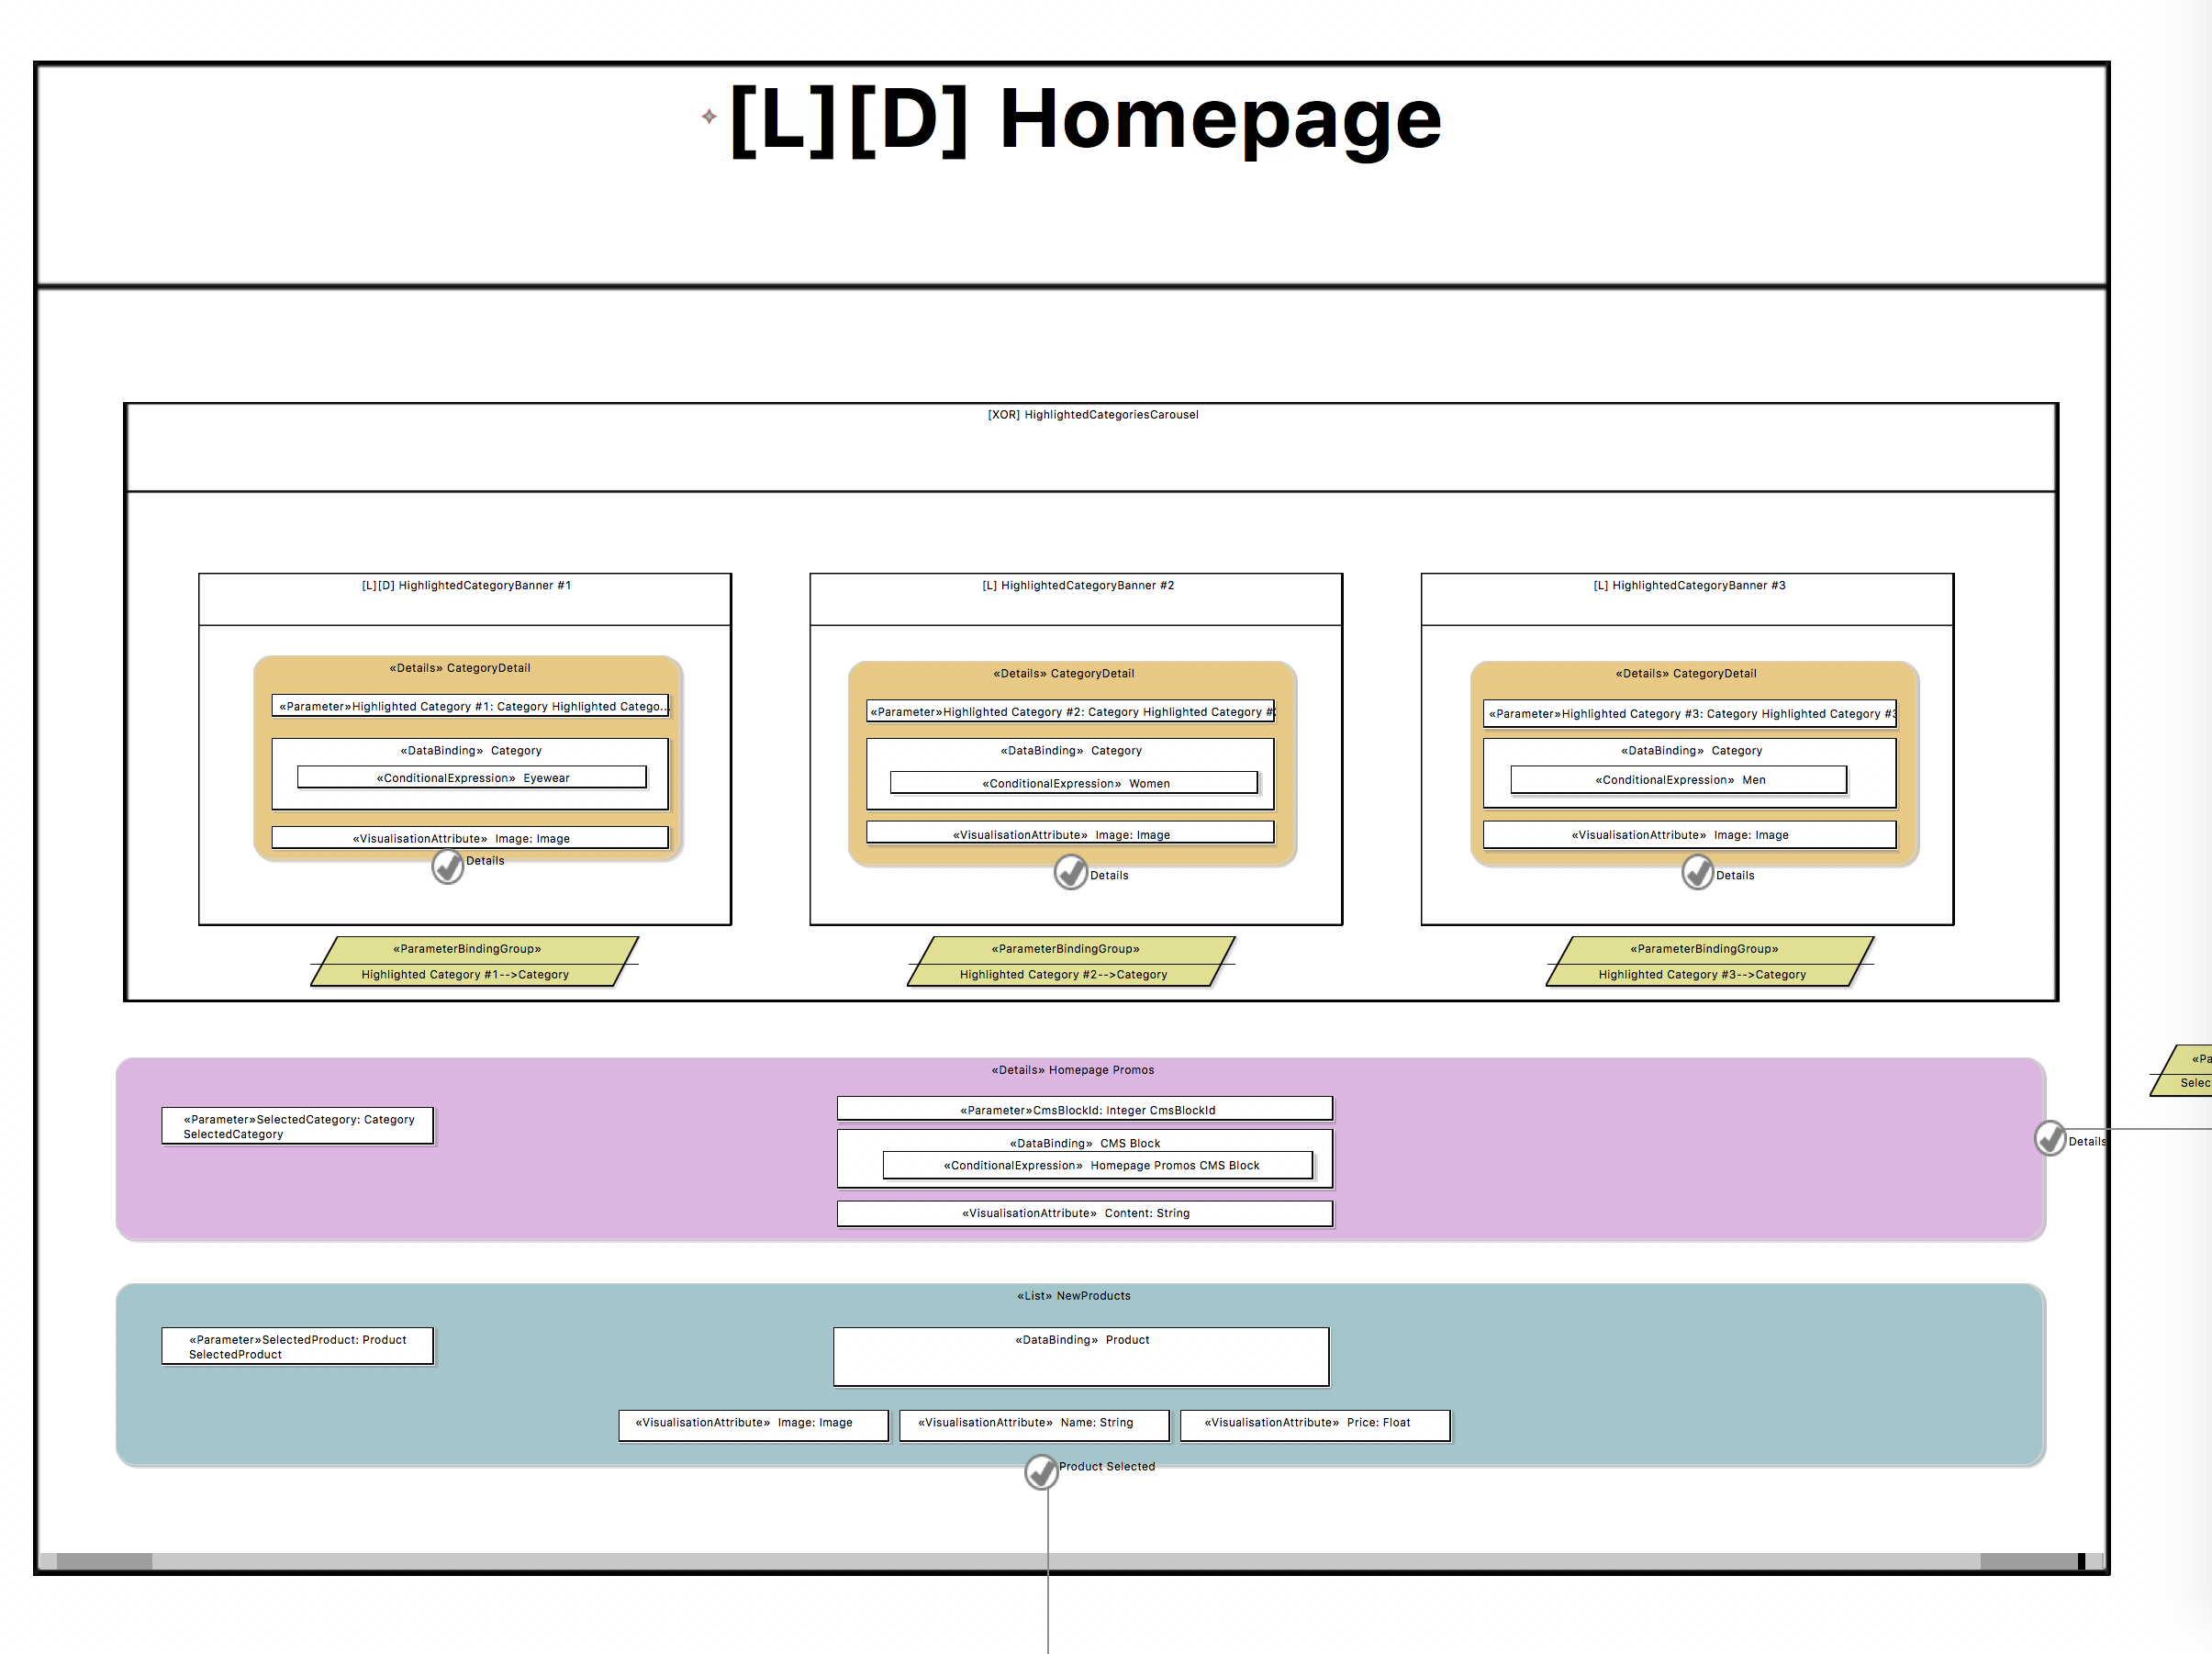
\includegraphics[height=7cm]{images/diagrams/before/ifml-homepage.png}
  \caption{Homepage IFML Diagram}
  \label{fig:ifml-before-homepage}
\end{figure}
\vspace{0.5cm}

\newpage
The following snippet of code is an extract from the IFML Model for the first \textit{HighlighedCategoryBanner View Container} element: 
\vspace{0.5cm}
\lstset{language=XML}
\begin{lstlisting} 
      <viewElements xsi:type="ext:Details"  name="CategoryDetail">
        <parameters  name="Highlighted Category #1" direction="inout">
          <constraints  language="SQL" body="Category.ID=18"/>
          <type xsi:type="uml:Class" href="model.uml#__W1boJ6PEeGdnpRmAZh-dQ"/>
        </parameters>
        <viewElementEvents xsi:type="ext:OnSelectEvent"  name="Details" viewElement="//@interactionFlowModel/@interactionFlowModelElements.0/@viewElements.0/@viewElements.0">
          <outInteractionFlows xsi:type="core:NavigationFlow"  targetInteractionFlowElement="//@interactionFlowModel/@interactionFlowModelElements.6">
            <parameterBindingGroup >
              <parameterBindings  sourceParameter="//@interactionFlowModel/@interactionFlowModelElements.0/@viewElements.0/@viewElements.0/@viewElements.0/@parameters.0" targetParameter="//@interactionFlowModel/@interactionFlowModelElements.6/@parameters.0"/>
            </parameterBindingGroup>
          </outInteractionFlows>
        </viewElementEvents>
        <viewComponentParts xsi:type="core:DataBinding"  name="Category" uniformResourceIdentifier="">
          <subViewComponentParts xsi:type="core:ConditionalExpression"  language="SQL" body="Category.ID=18" name="Eyewear"/>
        </viewComponentParts>
        <viewComponentParts xsi:type="core:VisualizationAttribute"  name="Image" featureConcept="//@domainModel/@domainElements.4"/>
      </viewElements>
    </viewElements>
\end{lstlisting}

\newpage
The above snippet belongs to a more complex IFML model hierarchy as shown in \ref{fig:ifml-before-hierarchy-homepage}.

\vspace{0.5cm}
\begin{figure}[H]
  \centering
    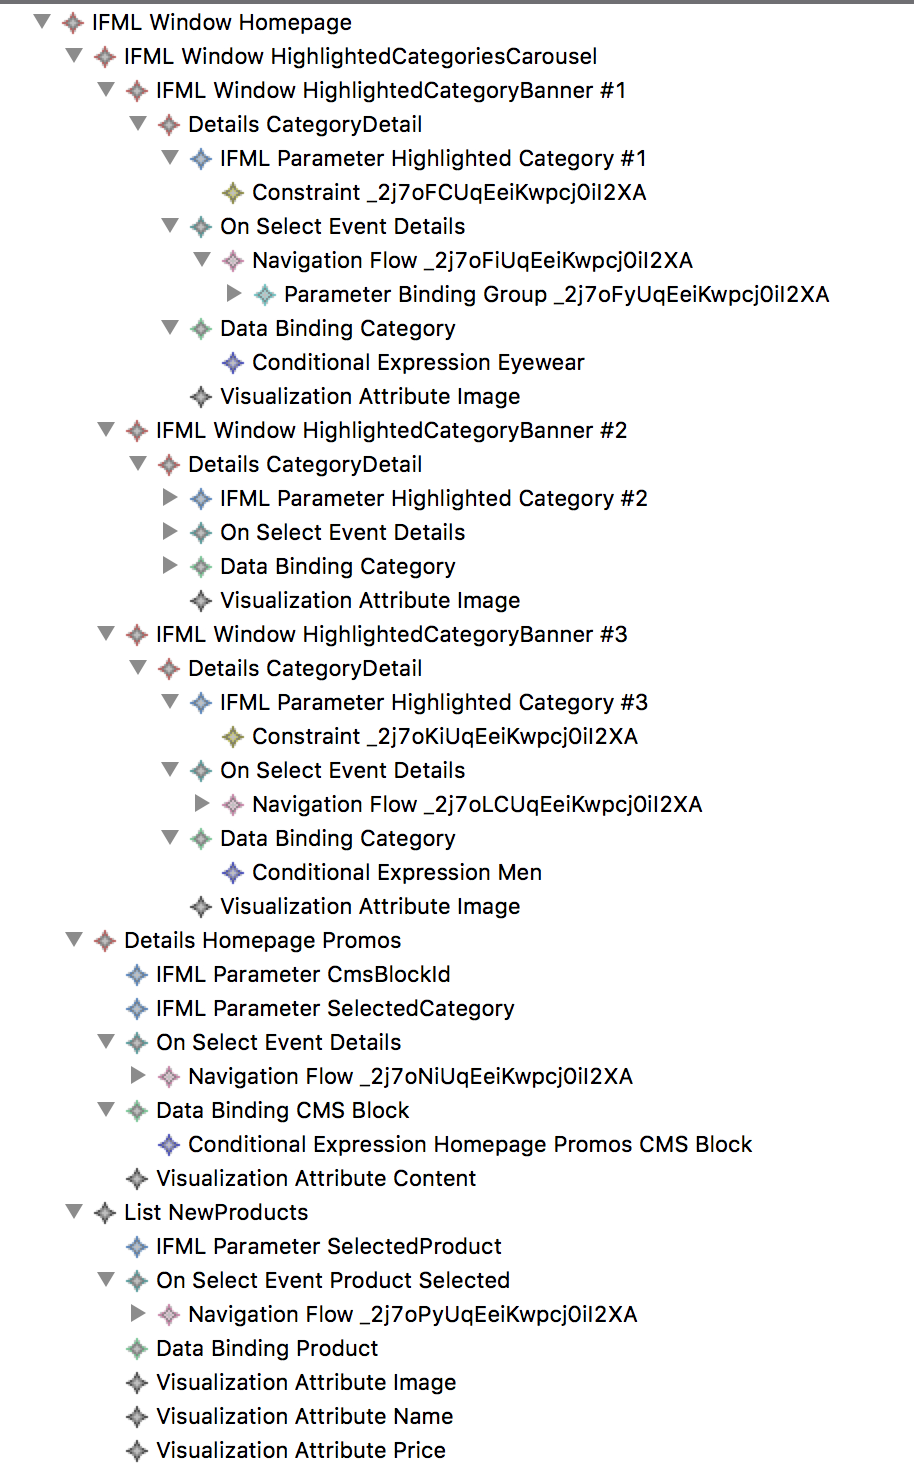
\includegraphics[height=12cm]{images/diagrams/before/ifml-hierarchy-homepage.png}
  \caption{Interaction Flow Homepage Model eCore representation}
  \label{fig:ifml-before-hierarchy-homepage}
\end{figure}
\vspace{0.5cm}

\subsubsection{Category Page overview}

The Madison Island Interaction Model for the Category Page (Figure \ref{fig:desktop-before-category} and \ref{fig:ifml-before-category}) is composed by a parent \textit{IFMLWindow} element in \textit{XOR mode} which presents information about the current category on the top of the page. Depending on the display mode property for the Category Entity, the user can be presented with two different \textit{View Containers} that are respectively activated using different \textit{Activation Expressions} based on the value of the property itself. Whilst the first scenario presents a \textit{Detail View Component} attached to a linked CMS Block, the second option shows two children view components representing both the filter sidebar and the products listing section with this last one having multiple \textit{Visualization Attribute} children nodes indicating the user is presented with an image used as thumbnail, a name and a price for each product belonging to the category shown.

\vspace{0.5cm}
\begin{figure}[H]
  \centering
  \subfloat[Display Mode PAGE]{{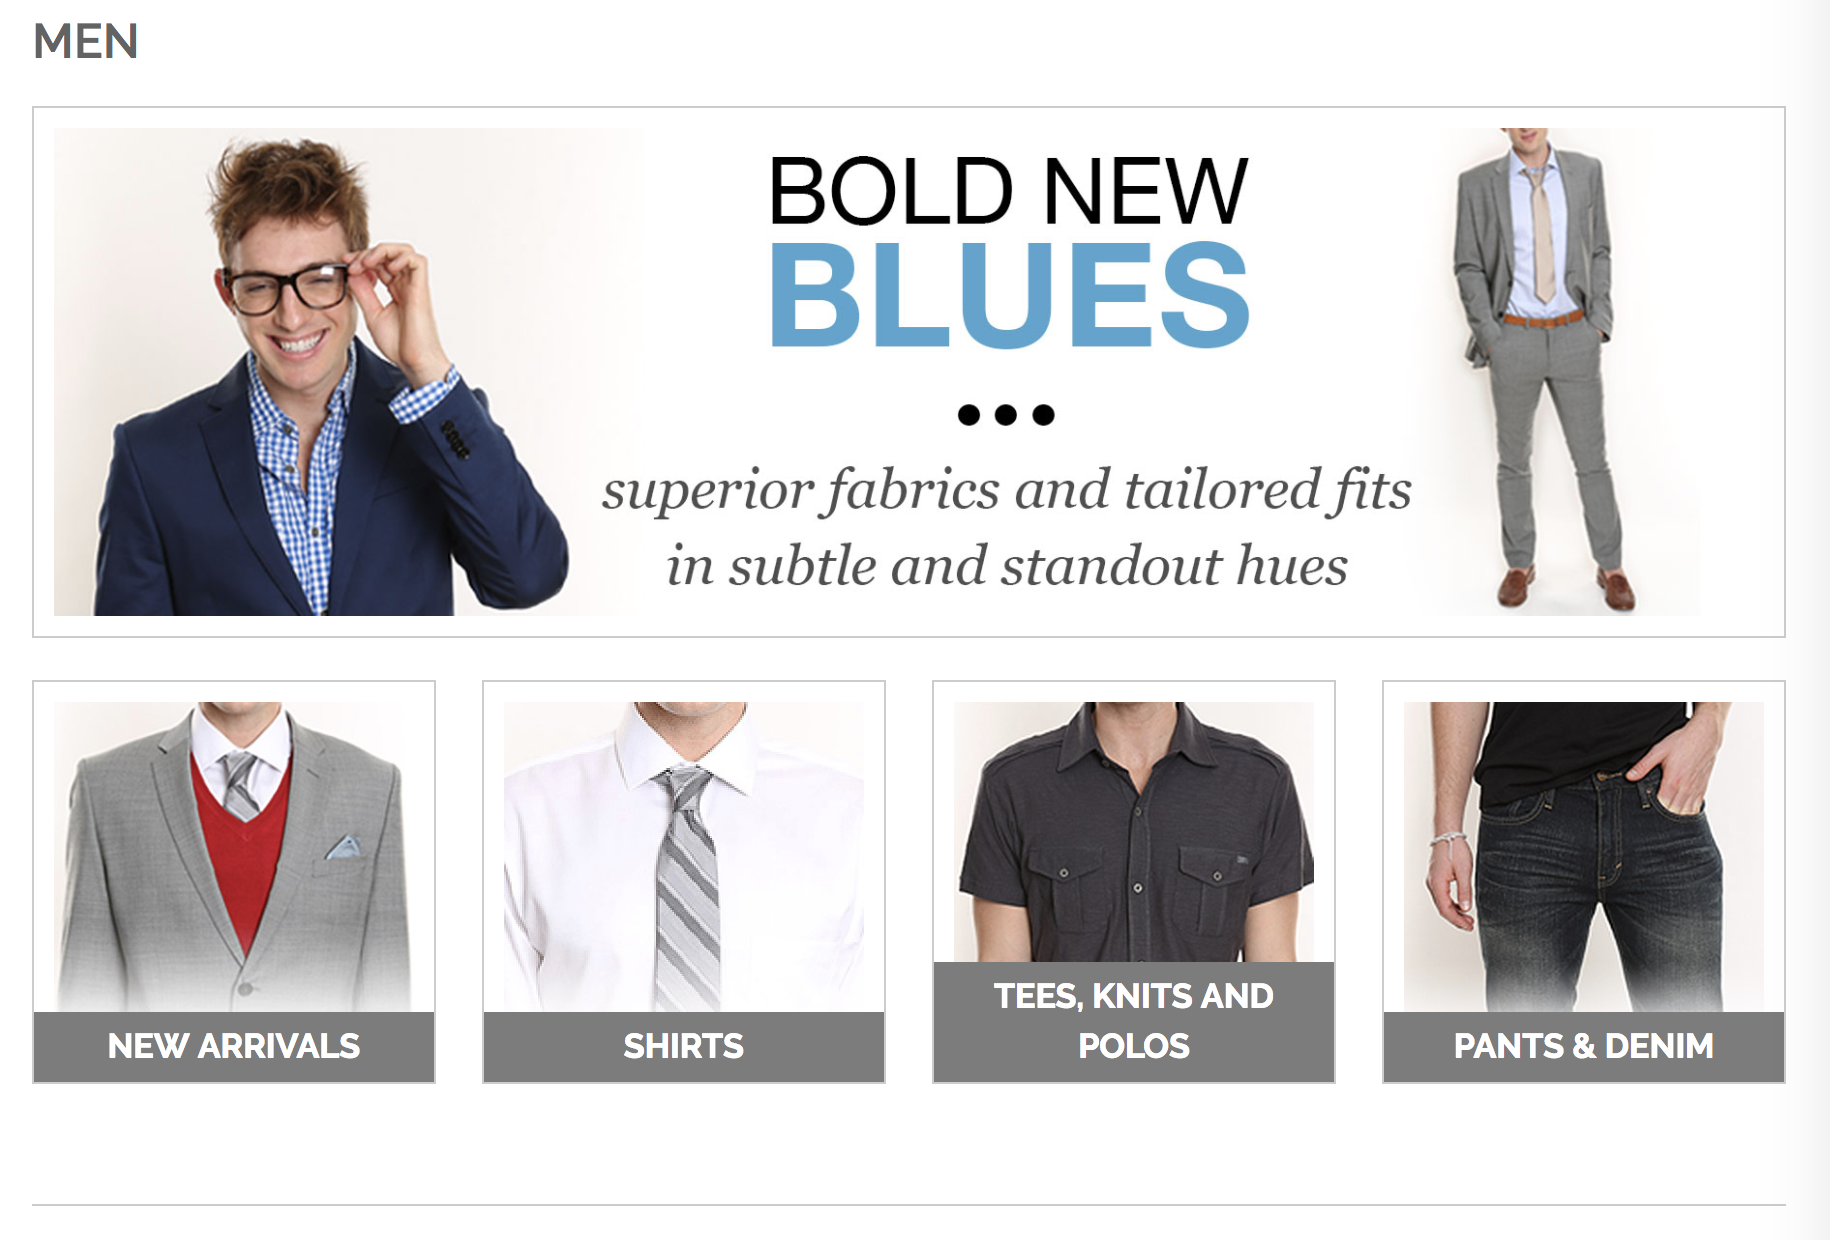
\includegraphics[width=7cm]{images/diagrams/before/desktop-category1.png} }}%
  \qquad
  \subfloat[Display Mode PRODUCTS]{{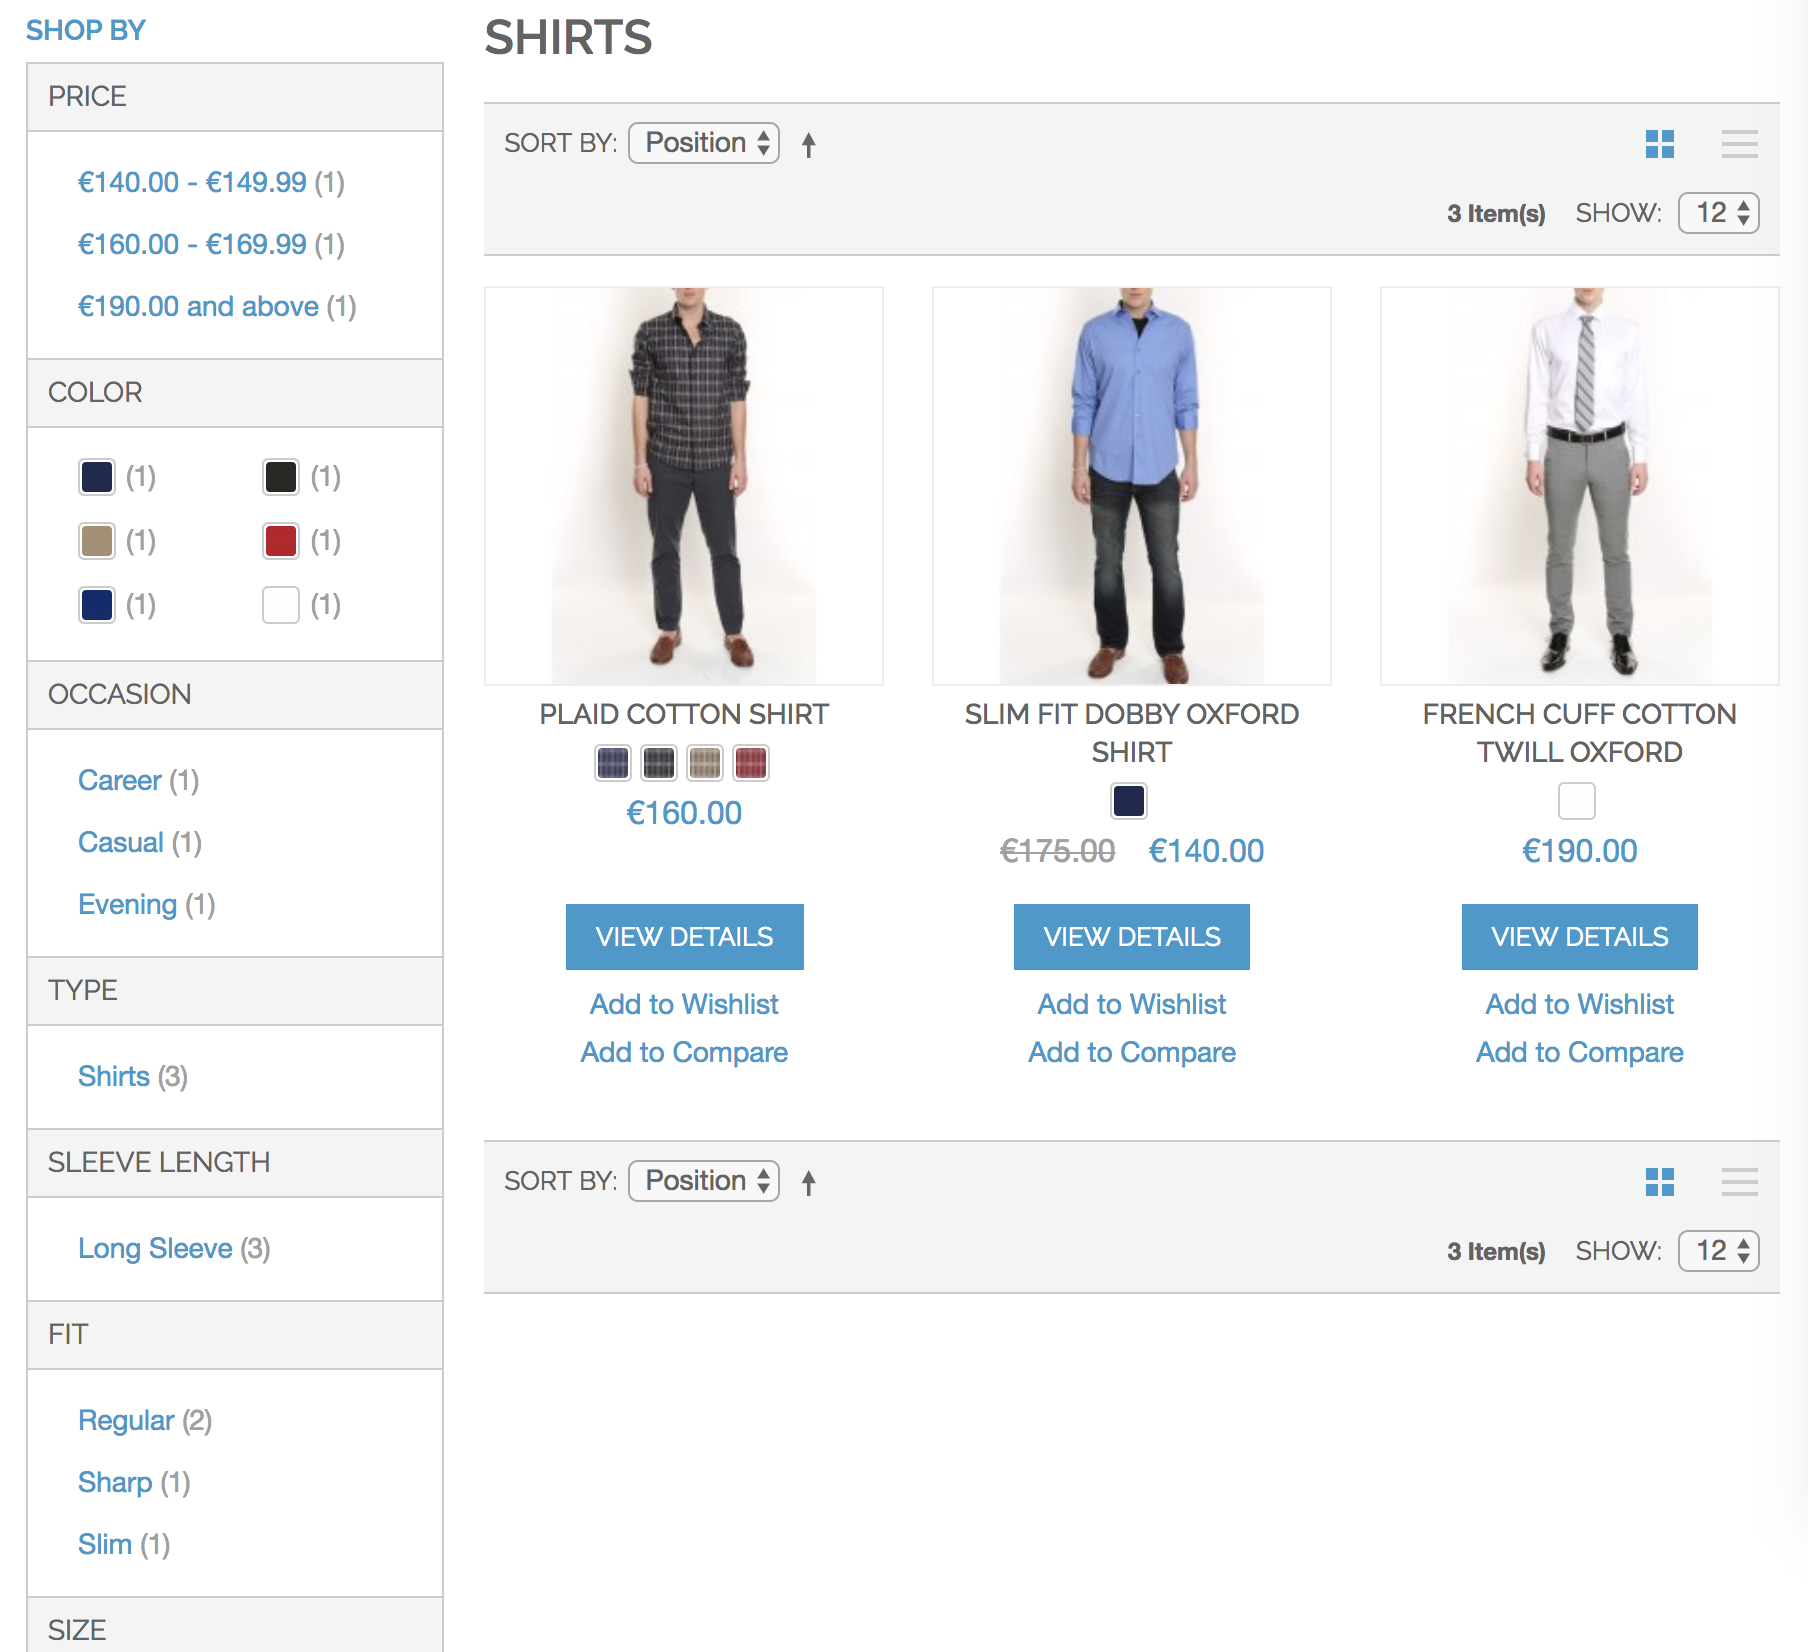
\includegraphics[width=7cm]{images/diagrams/before/desktop-category2.png} }}%
  \caption{Category Desktop Versions}%
  \label{fig:desktop-before-category}%
\end{figure}

\begin{figure}[H]
  \centering
    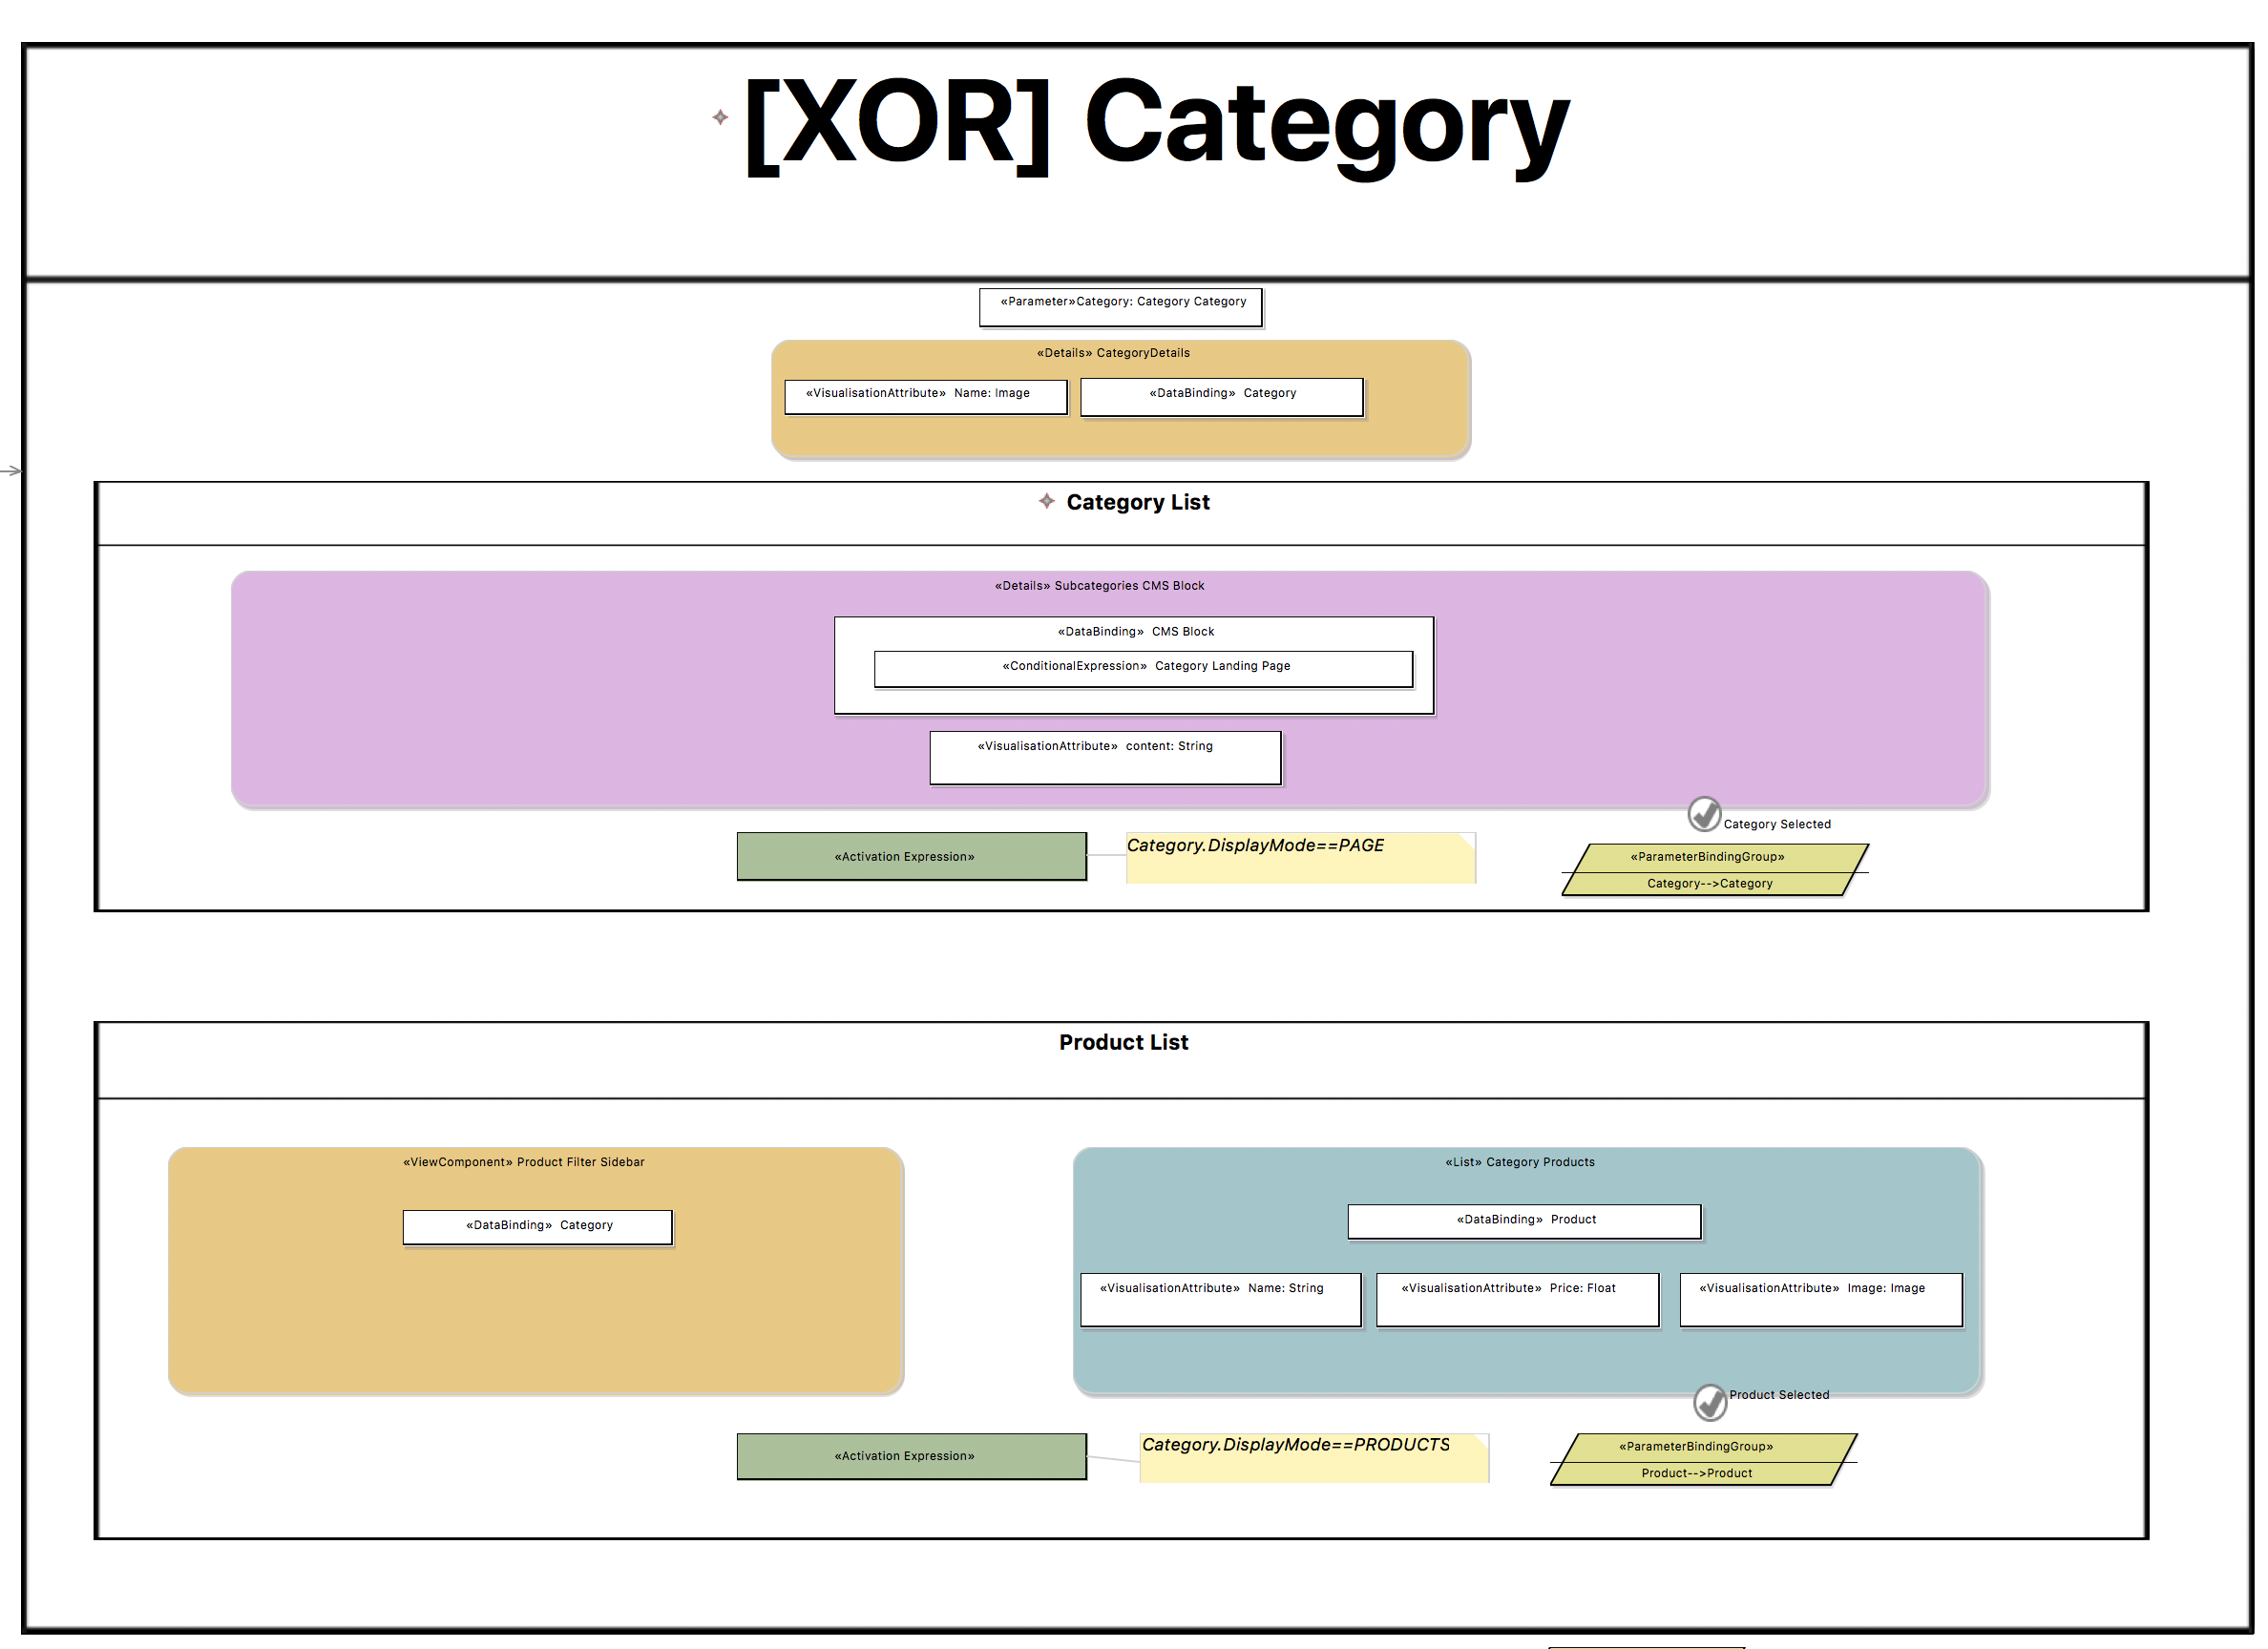
\includegraphics[height=10cm]{images/diagrams/before/ifml-category.png}
  \caption{Category IFML Diagram}
  \label{fig:ifml-before-category}
\end{figure}
\vspace{0.5cm}

The IFML Model code for the first \textit{Category Products List} element we just described has this form: 
\vspace{0.5cm}
\lstset{language=XML}
\begin{lstlisting} 
    <viewElements xsi:type="ext:List"  name="Category Products">
    <viewElementEvents xsi:type="ext:OnSelectEvent"  name="Product Selected" viewElement="//@interactionFlowModel/@interactionFlowModelElements.6/@viewElements.1/@viewElements.0">
      <outInteractionFlows xsi:type="core:NavigationFlow"  targetInteractionFlowElement="//@interactionFlowModel/@interactionFlowModelElements.1">
        <parameterBindingGroup >
          <parameterBindings  sourceParameter="//@interactionFlowModel/@interactionFlowModelElements.1/@parameters.0" targetParameter="//@interactionFlowModel/@interactionFlowModelElements.1/@parameters.0"/>
        </parameterBindingGroup>
      </outInteractionFlows>
    </viewElementEvents>
    <viewComponentParts xsi:type="core:DataBinding"  name="Product" domainConcept="//@domainModel/@domainElements.3">
      <conditionalExpression  language="SQL" body="Category IN Product.Categories" name="Category Products"/>
    </viewComponentParts>
    <viewComponentParts xsi:type="core:VisualizationAttribute"  name="Image" featureConcept="//@domainModel/@domainElements.7"/>
    <viewComponentParts xsi:type="core:VisualizationAttribute"  name="Name" featureConcept="//@domainModel/@domainElements.8"/>
    <viewComponentParts xsi:type="core:VisualizationAttribute"  name="Price" featureConcept="//@domainModel/@domainElements.9"/>
  </viewElements>
  <viewElements xsi:type="core:ViewComponent"  name="Product Filter Sidebar">
    <viewComponentParts xsi:type="core:DataBinding"  name="Category"/>
  </viewElements>
</viewElements>
\end{lstlisting}

\newpage
The full expanded model hierarchy for the \textit{IFMLWindow} Category element is shown in Figure \ref{fig:ifml-before-hierarchy-category}.

\vspace{0.5cm}
\begin{figure}[H]
  \centering
    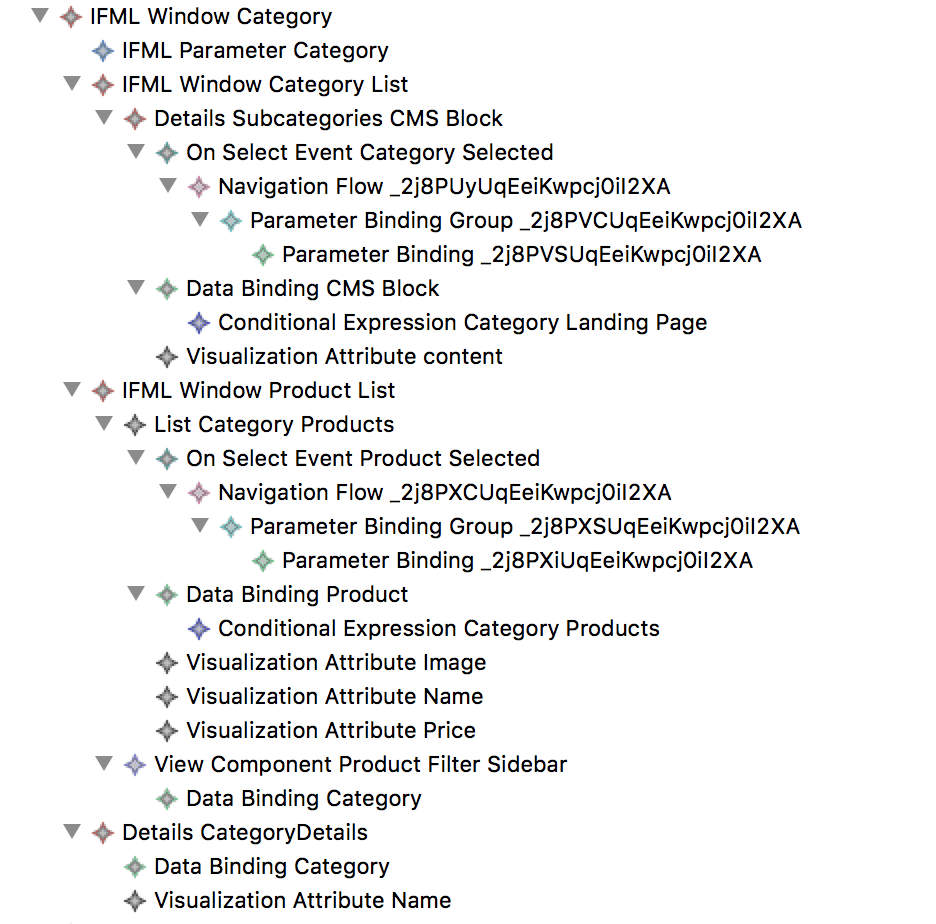
\includegraphics[width=13cm]{images/diagrams/before/ifml-hierarchy-category.png}
  \caption{Interaction Flow Category Model eCore representation}
  \label{fig:ifml-before-hierarchy-category}
\end{figure}
\vspace{0.5cm}


\subsubsection{Product Page overview}

The Madison Island Interaction Model for the Product page (Figure \ref{fig:desktop-before-product} and \ref{fig:ifml-before-product}) is mainly built with a single \textit{IFMLWindow} element containing different types of \textit{View Component} nodes with the main one being a Detail type one bound to the current product data entity. The other two elements are the single \textit{Form View Component} descibing the Add to Cart section and its possible interactions and the \textit{List View Component} holding the information for the Related Product widget.

\newpage
\vspace{0.5cm}
\begin{figure}[H]
  \centering
    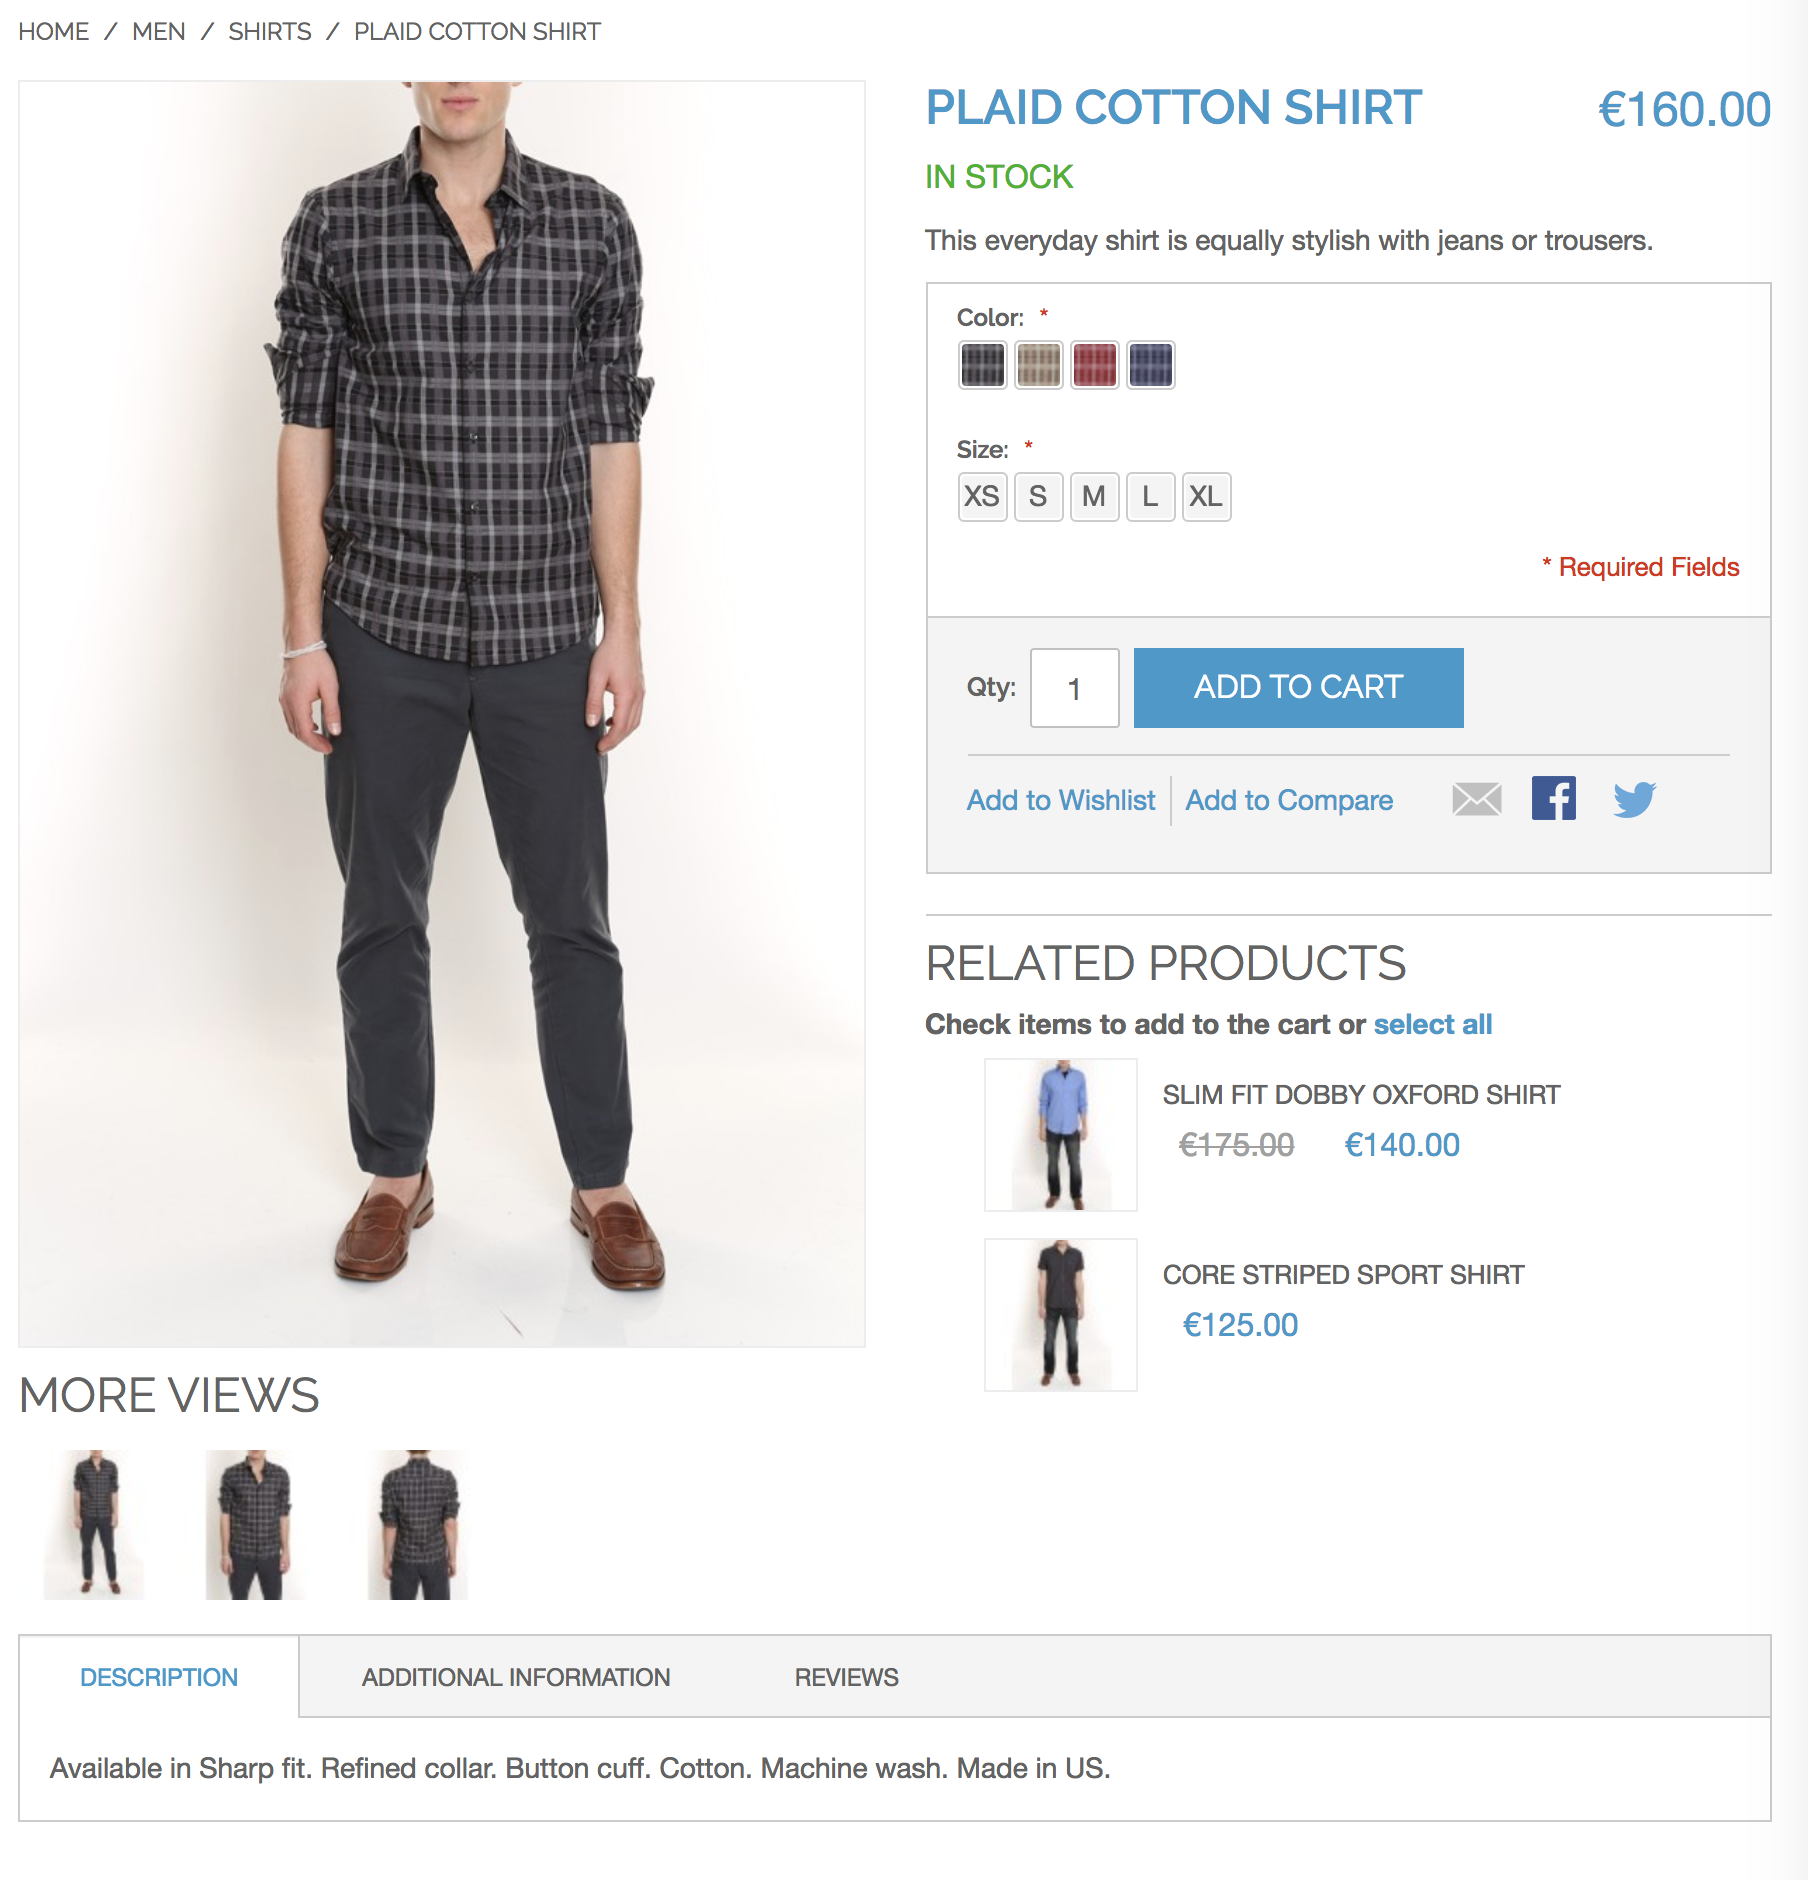
\includegraphics[height=10cm]{images/diagrams/before/desktop-product.png}
  \caption{Product Page Desktop Version}
  \label{fig:desktop-before-product}
\end{figure}

\vspace{0.5cm}
\begin{figure}[H]
  \centering
    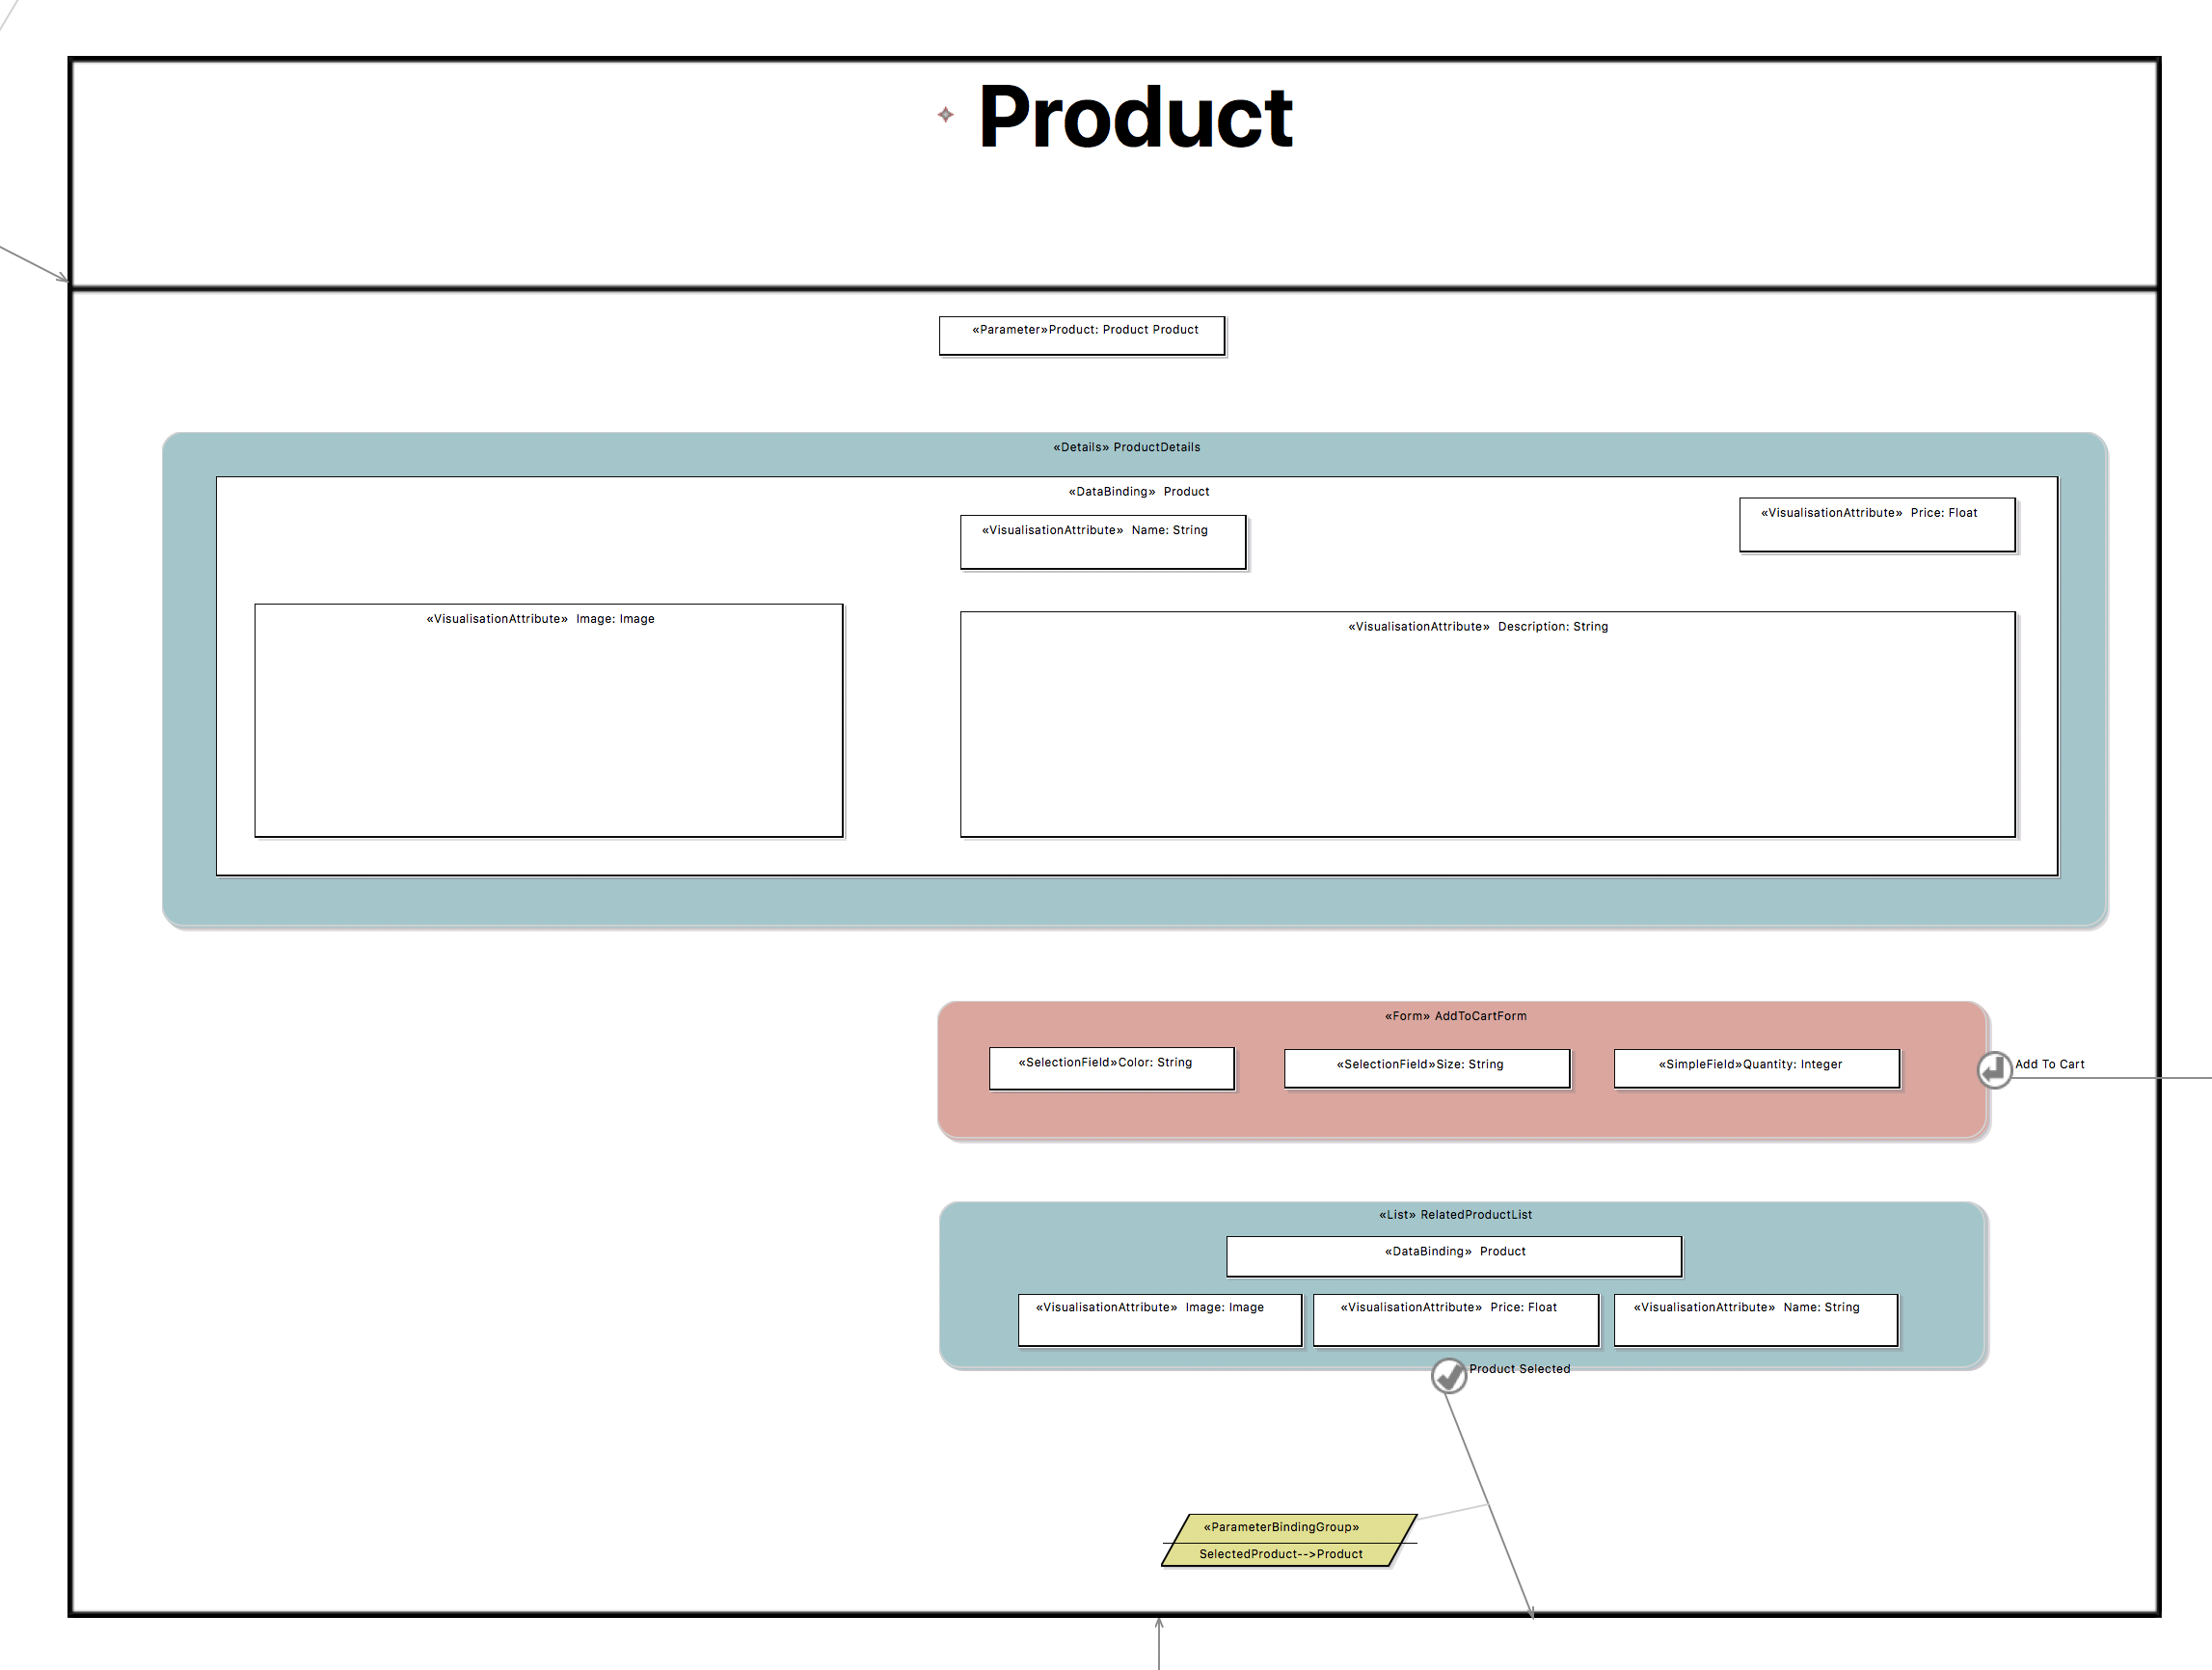
\includegraphics[height=10cm]{images/diagrams/before/ifml-product.png}
  \caption{Product Page IFML Diagram}
  \label{fig:ifml-before-product}
\end{figure}
\vspace{0.5cm}

\newpage
The structure of the model just outlined produces the following IFMLModel code:
\vspace{0.5cm}
\lstset{language=XML}
\begin{lstlisting} 
    <interactionFlowModelElements xsi:type="ext:IFMLWindow"  name="Product" inInteractionFlows="//@interactionFlowModel/@interactionFlowModelElements.1/@viewElements.2/@viewElementEvents.0/@outInteractionFlows.0 //@interactionFlowModel/@interactionFlowModelElements.0/@viewElements.2/@viewElementEvents.0/@outInteractionFlows.0 //@interactionFlowModel/@interactionFlowModelElements.10/@viewElements.0/@viewElementEvents.0/@outInteractionFlows.0 //@interactionFlowModel/@interactionFlowModelElements.6/@viewElements.1/@viewElements.0/@viewElementEvents.0/@outInteractionFlows.0">
      <parameters  name="Product">
        <type xsi:type="uml:Class" href="model.uml#_nyxiEA9LEeiZ14TmPBeBNA"/>
      </parameters>
      <viewElements xsi:type="ext:Details"  name="ProductDetails">
        <viewComponentParts xsi:type="core:DataBinding"  name="Product" uniformResourceIdentifier="">
          <subViewComponentParts xsi:type="core:VisualizationAttribute"  name="Price" featureConcept="//@domainModel/@domainElements.9"/>
          <subViewComponentParts xsi:type="core:VisualizationAttribute"  name="Image" featureConcept="//@domainModel/@domainElements.7"/>
          <subViewComponentParts xsi:type="core:VisualizationAttribute"  name="Name" featureConcept="//@domainModel/@domainElements.8"/>
          <subViewComponentParts xsi:type="core:VisualizationAttribute"  name="Description" featureConcept="//@domainModel/@domainElements.10"/>
        </viewComponentParts>
      </viewElements>
      <viewElements xsi:type="ext:Form"  name="AddToCartForm">
        <viewElementEvents xsi:type="ext:OnSubmitEvent"  name="Add To Cart" viewElement="//@interactionFlowModel/@interactionFlowModelElements.1/@viewElements.1">
          <outInteractionFlows xsi:type="core:NavigationFlow"  targetInteractionFlowElement="//@interactionFlowModel/@interactionFlowModelElements.9">
            <parameterBindingGroup >
              <parameterBindings  sourceParameter="//@interactionFlowModel/@interactionFlowModelElements.1/@viewElements.1/@viewComponentParts.2" targetParameter="//@interactionFlowModel/@interactionFlowModelElements.1/@viewElements.1/@viewComponentParts.2"/>
            </parameterBindingGroup>
          </outInteractionFlows>
        </viewElementEvents>
        <viewComponentParts xsi:type="ext:SelectionField"  name="Color">
          <type xsi:type="uml:PrimitiveType" href="model.uml#_VK2hkJ6QEeGdnpRmAZh-dQ"/>
        </viewComponentParts>
        <viewComponentParts xsi:type="ext:SelectionField"  name="Size">
          <type xsi:type="uml:PrimitiveType" href="model.uml#_VK2hkJ6QEeGdnpRmAZh-dQ"/>
        </viewComponentParts>
        <viewComponentParts xsi:type="ext:SimpleField"  name="Quantity">
          <type xsi:type="uml:PrimitiveType" href="model.uml#_YGTmEJ6QEeGdnpRmAZh-dQ"/>
        </viewComponentParts>
      </viewElements>
      <viewElements xsi:type="ext:List"  name="RelatedProductList">
        <viewElementEvents xsi:type="ext:OnSelectEvent"  name="Product Selected" viewElement="//@interactionFlowModel/@interactionFlowModelElements.1/@viewElements.2">
          <outInteractionFlows xsi:type="core:NavigationFlow"  targetInteractionFlowElement="//@interactionFlowModel/@interactionFlowModelElements.1">
            <parameterBindingGroup >
              <parameterBindings  sourceParameter="//@interactionFlowModel/@interactionFlowModelElements.0/@viewElements.2/@parameters.0" targetParameter="//@interactionFlowModel/@interactionFlowModelElements.1/@parameters.0"/>
            </parameterBindingGroup>
          </outInteractionFlows>
        </viewElementEvents>
        <viewComponentParts xsi:type="core:DataBinding"  name="Product"/>
        <viewComponentParts xsi:type="core:VisualizationAttribute"  name="Image" featureConcept="//@domainModel/@domainElements.7"/>
        <viewComponentParts xsi:type="core:VisualizationAttribute"  name="Name" featureConcept="//@domainModel/@domainElements.8"/>
        <viewComponentParts xsi:type="core:VisualizationAttribute"  name="Price" featureConcept="//@domainModel/@domainElements.9"/>
      </viewElements>
    </interactionFlowModelElements>
\end{lstlisting}

\newpage
The model representation of this Product page structure is shown in Figure \ref{fig:ifml-before-hierarchy-product}

\vspace{0.5cm}
\begin{figure}[H]
  \centering
    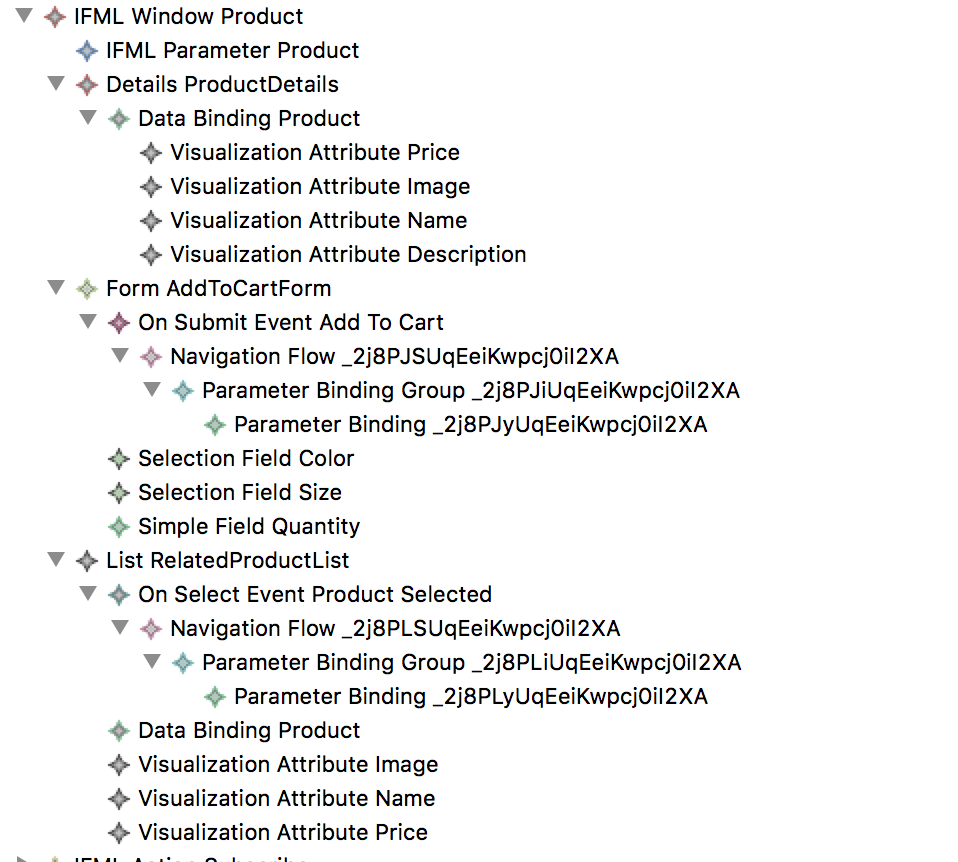
\includegraphics[width=13cm]{images/diagrams/before/ifml-hierarchy-product.png}
  \caption{Interaction Flow Product Model eCore representation}
  \label{fig:ifml-before-hierarchy-product}
\end{figure}
\vspace{0.5cm}

\subsubsection{Shopping Cart Page overview}
\label{shopping-cart-page-overview}
The Madison Island Interaction Model for the Shopping Cart page (Figure \ref{fig:desktop-before-shoppingcart} and \ref{fig:ifml-before-shoppingcart}) is  built with a single \textit{IFMLWindow} landmark container (flagging it as accessible from everywhere) including multiple \textit{Form View Component} instances representing the sidebar interactions with the discount codes and shipping estimation widgets. Besides the sidebar, the area with the cart status and the items in the cart is shown with another \textit{Form View Component} controlled by the \textit{Activation Condition} responsible for showing items when cart is not empty only. The area is modeled with a Form component because of the Qty input text fields which allow the user to update the related item quantities or empty the whole cart at any time. Both these interactions are controlled with specific \textit{IFMLAction} elements triggered on these \textit{Events}.

\newpage
\vspace{0.5cm}
\begin{figure}[H]
  \centering
    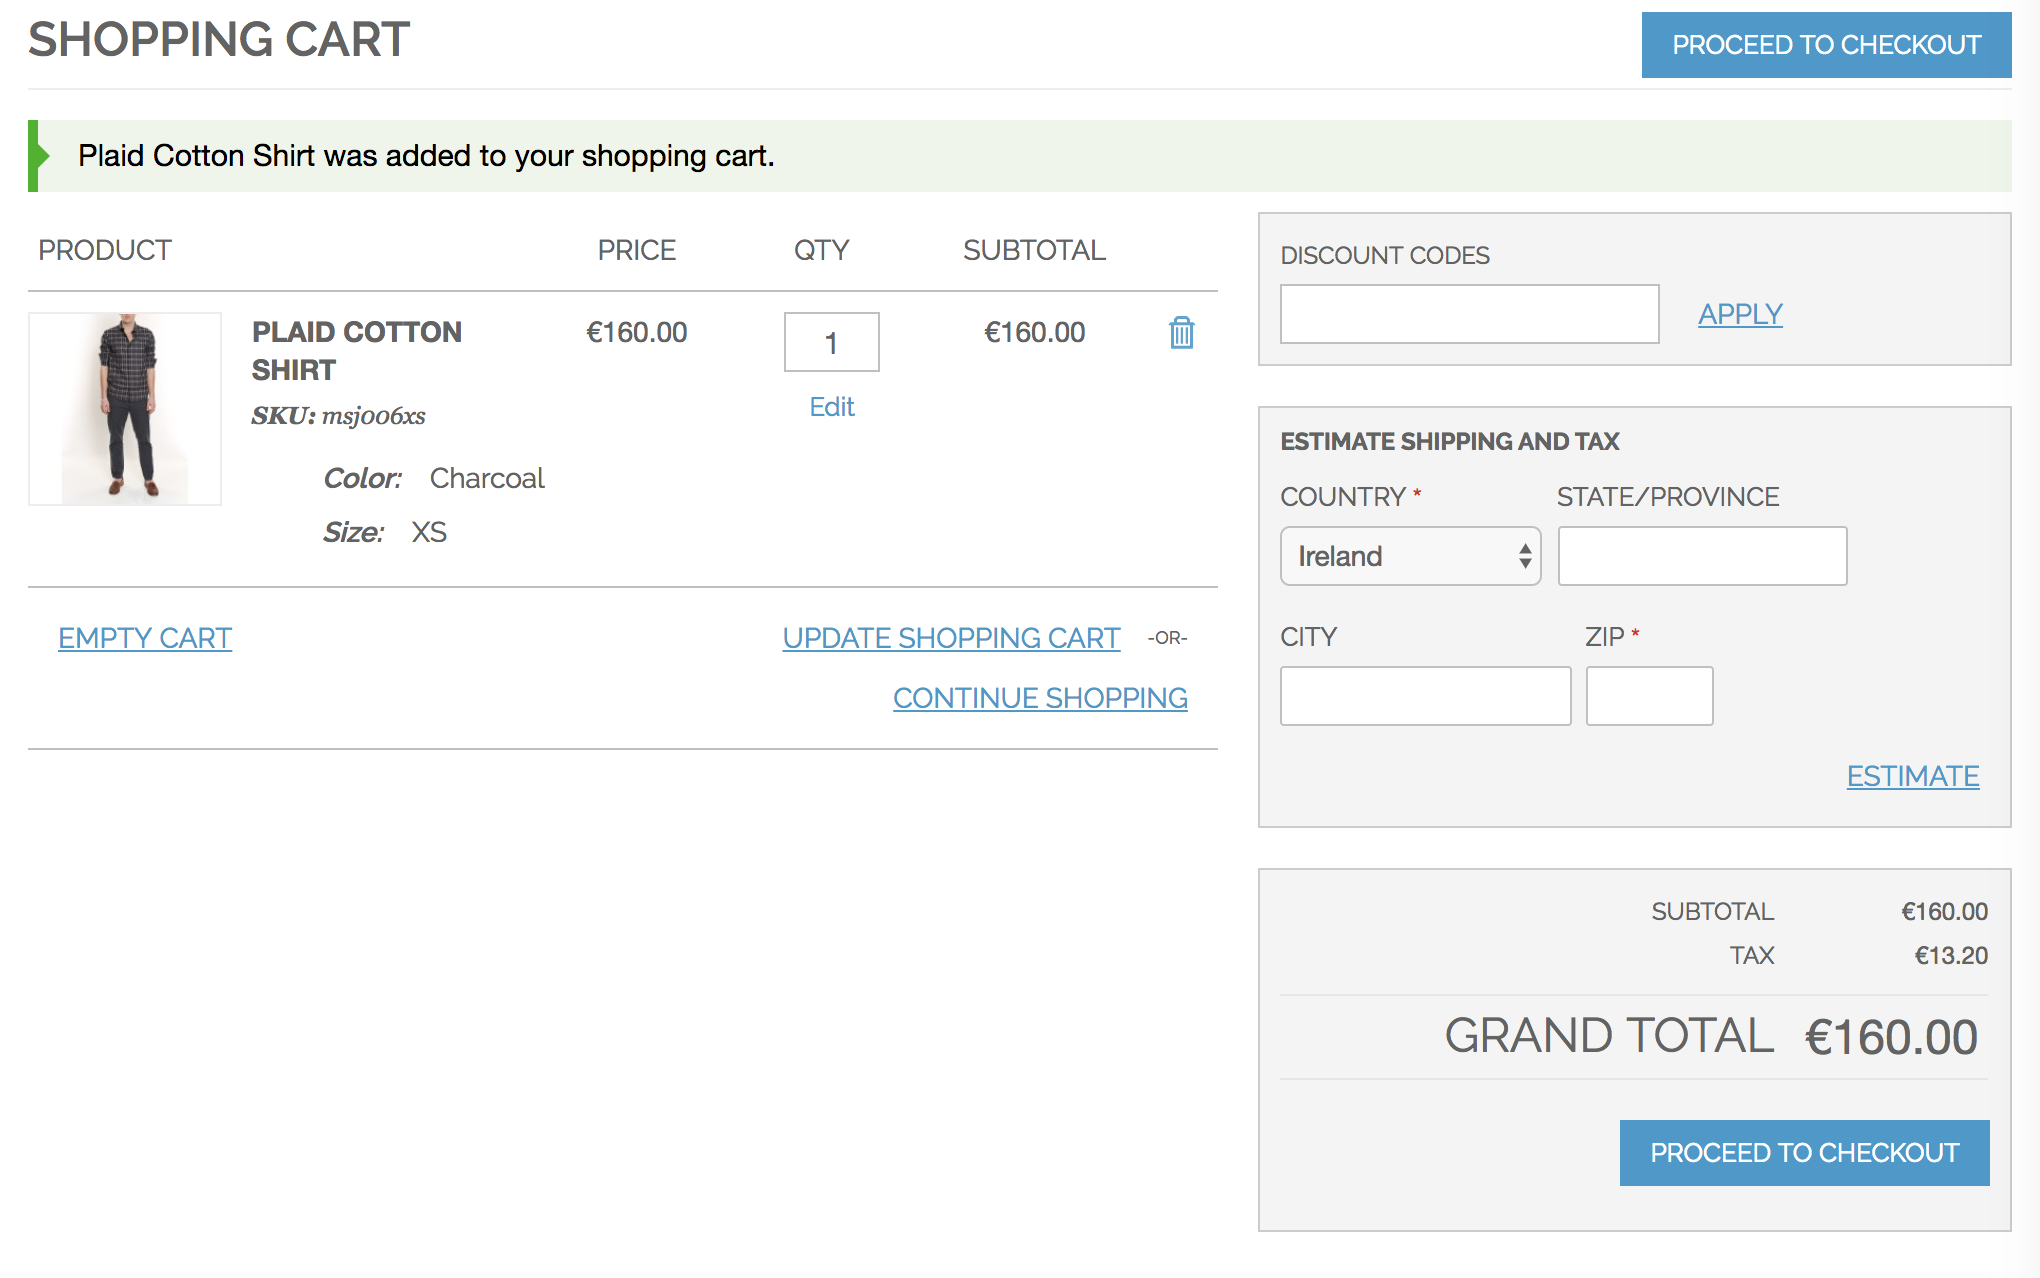
\includegraphics[height=10cm]{images/diagrams/before/desktop-shoppingcart.png}
  \caption{Shopping Cart Page Desktop Version}
  \label{fig:desktop-before-shoppingcart}
\end{figure}

\vspace{0.5cm}
\begin{figure}[H]
  \centering
    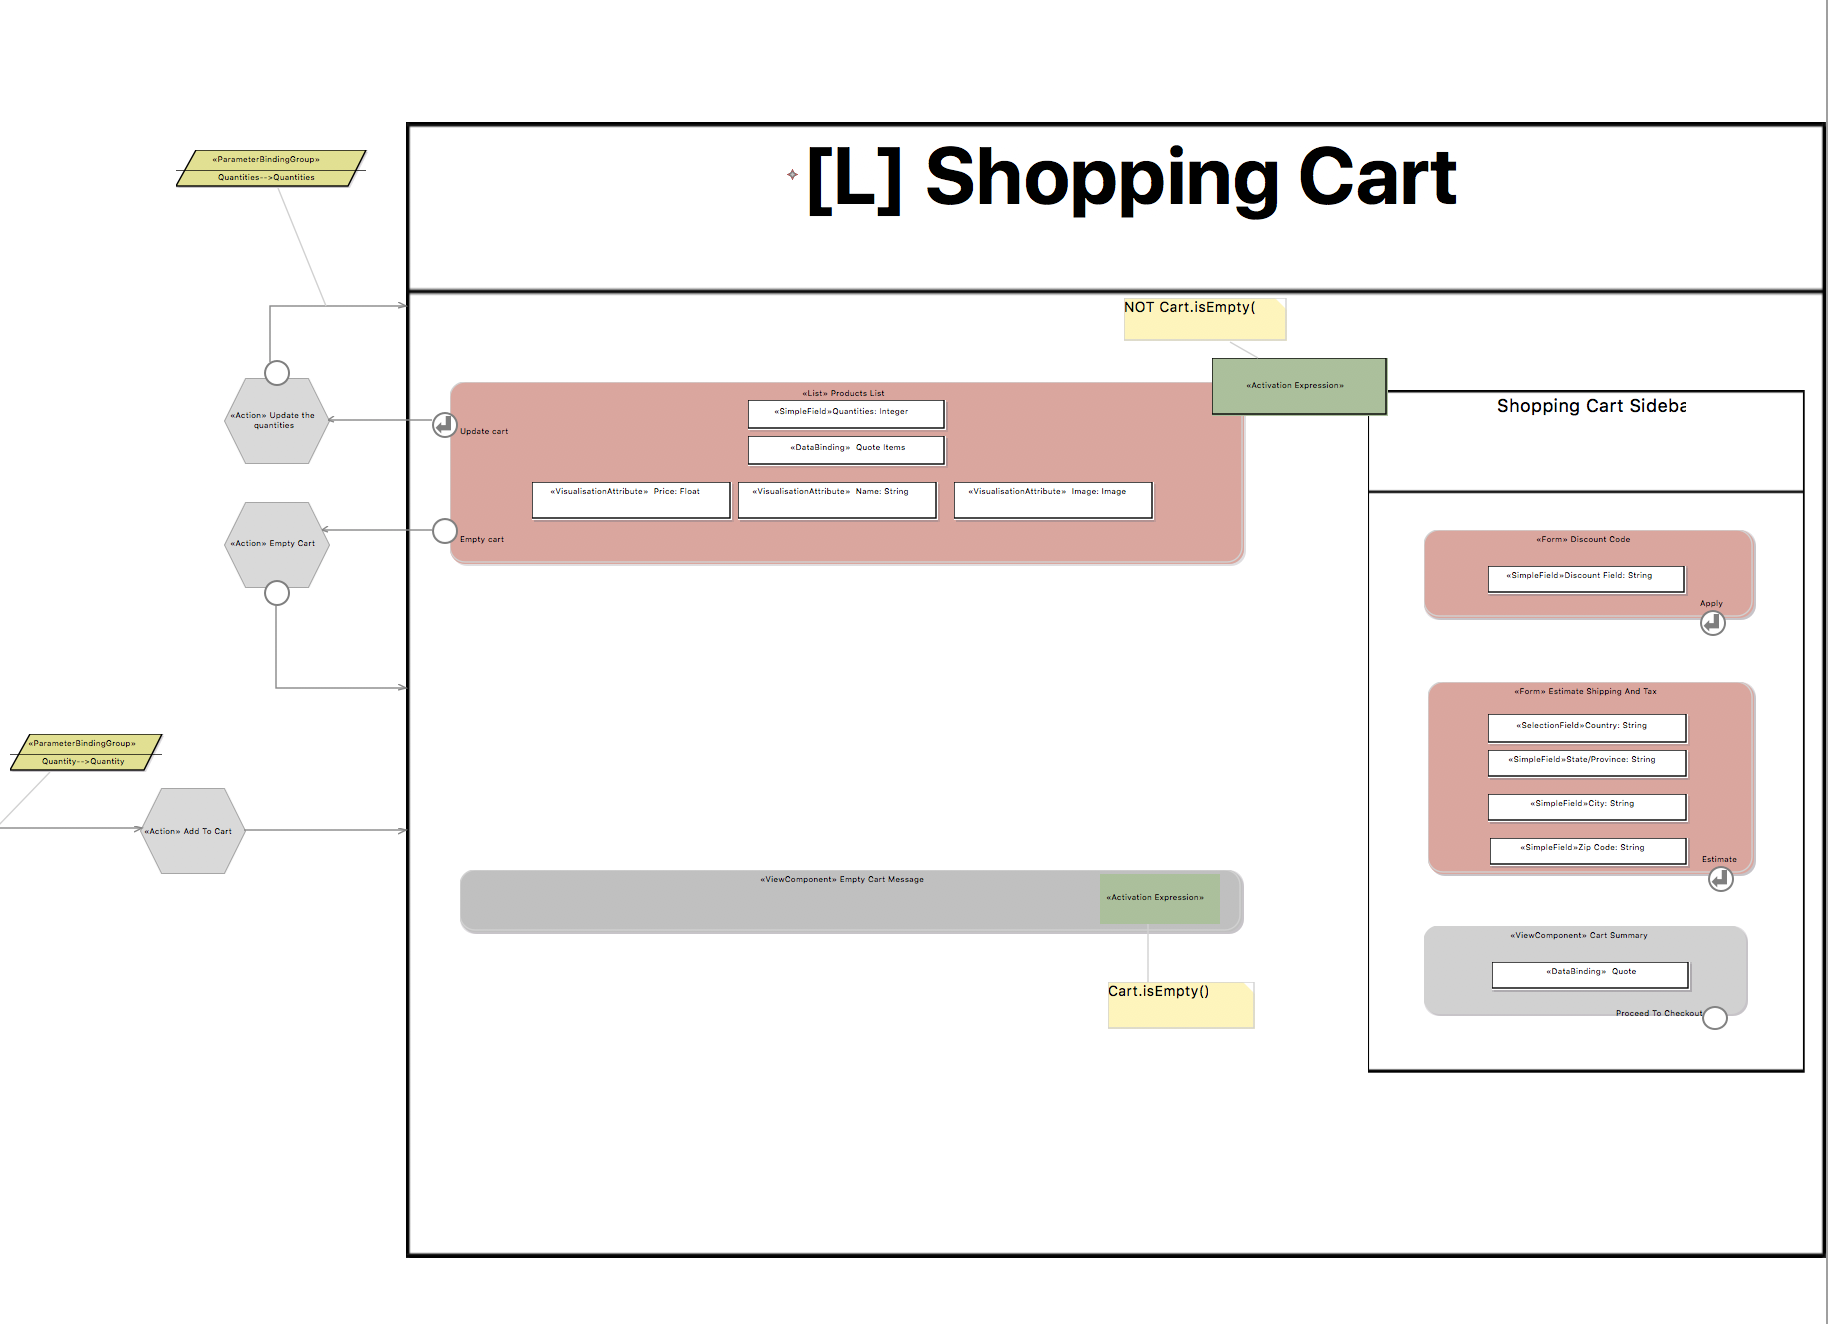
\includegraphics[height=10cm]{images/diagrams/before/ifml-shoppingcart.png}
  \caption{Shopping Cart Page IFML Diagram}
  \label{fig:ifml-before-shoppingcart}
\end{figure}
\vspace{0.5cm}

\newpage
As per shown in Figure \ref{fig:ifml-before-hierarchy-shoppingcart}, the Interaction Flow model representing the shopping page has the following form:
\vspace{0.5cm}
\lstset{language=XML}
\begin{lstlisting} 
    <interactionFlowModelElements xsi:type="ext:IFMLWindow"  name="Product" inInteractionFlows="//@interactionFlowModel/@interactionFlowModelElements.1/@viewElements.2/@viewElementEvents.0/@outInteractionFlows.0 //@interactionFlowModel/@interactionFlowModelElements.0/@viewElements.2/@viewElementEvents.0/@outInteractionFlows.0 //@interactionFlowModel/@interactionFlowModelElements.10/@viewElements.0/@viewElementEvents.0/@outInteractionFlows.0 //@interactionFlowModel/@interactionFlowModelElements.6/@viewElements.1/@viewElements.0/@viewElementEvents.0/@outInteractionFlows.0">
      <parameters  name="Product">
        <type xsi:type="uml:Class" href="model.uml#_nyxiEA9LEeiZ14TmPBeBNA"/>
      </parameters>
      <viewElements xsi:type="ext:Details"  name="ProductDetails">
        <viewComponentParts xsi:type="core:DataBinding"  name="Product" uniformResourceIdentifier="">
          <subViewComponentParts xsi:type="core:VisualizationAttribute"  name="Price" featureConcept="//@domainModel/@domainElements.9"/>
          <subViewComponentParts xsi:type="core:VisualizationAttribute"  name="Image" featureConcept="//@domainModel/@domainElements.7"/>
          <subViewComponentParts xsi:type="core:VisualizationAttribute"  name="Name" featureConcept="//@domainModel/@domainElements.8"/>
          <subViewComponentParts xsi:type="core:VisualizationAttribute"  name="Description" featureConcept="//@domainModel/@domainElements.10"/>
        </viewComponentParts>
      </viewElements>
      <viewElements xsi:type="ext:Form"  name="AddToCartForm">
        <viewElementEvents xsi:type="ext:OnSubmitEvent"  name="Add To Cart" viewElement="//@interactionFlowModel/@interactionFlowModelElements.1/@viewElements.1">
          <outInteractionFlows xsi:type="core:NavigationFlow"  targetInteractionFlowElement="//@interactionFlowModel/@interactionFlowModelElements.9">
            <parameterBindingGroup >
              <parameterBindings  sourceParameter="//@interactionFlowModel/@interactionFlowModelElements.1/@viewElements.1/@viewComponentParts.2" targetParameter="//@interactionFlowModel/@interactionFlowModelElements.1/@viewElements.1/@viewComponentParts.2"/>
            </parameterBindingGroup>
          </outInteractionFlows>
        </viewElementEvents>
        <viewComponentParts xsi:type="ext:SelectionField"  name="Color">
          <type xsi:type="uml:PrimitiveType" href="model.uml#_VK2hkJ6QEeGdnpRmAZh-dQ"/>
        </viewComponentParts>
        <viewComponentParts xsi:type="ext:SelectionField"  name="Size">
          <type xsi:type="uml:PrimitiveType" href="model.uml#_VK2hkJ6QEeGdnpRmAZh-dQ"/>
        </viewComponentParts>
        <viewComponentParts xsi:type="ext:SimpleField"  name="Quantity">
          <type xsi:type="uml:PrimitiveType" href="model.uml#_YGTmEJ6QEeGdnpRmAZh-dQ"/>
        </viewComponentParts>
      </viewElements>
      <viewElements xsi:type="ext:List"  name="RelatedProductList">
        <viewElementEvents xsi:type="ext:OnSelectEvent"  name="Product Selected" viewElement="//@interactionFlowModel/@interactionFlowModelElements.1/@viewElements.2">
          <outInteractionFlows xsi:type="core:NavigationFlow"  targetInteractionFlowElement="//@interactionFlowModel/@interactionFlowModelElements.1">
            <parameterBindingGroup >
              <parameterBindings  sourceParameter="//@interactionFlowModel/@interactionFlowModelElements.0/@viewElements.2/@parameters.0" targetParameter="//@interactionFlowModel/@interactionFlowModelElements.1/@parameters.0"/>
            </parameterBindingGroup>
          </outInteractionFlows>
        </viewElementEvents>
        <viewComponentParts xsi:type="core:DataBinding"  name="Product"/>
        <viewComponentParts xsi:type="core:VisualizationAttribute"  name="Image" featureConcept="//@domainModel/@domainElements.7"/>
        <viewComponentParts xsi:type="core:VisualizationAttribute"  name="Name" featureConcept="//@domainModel/@domainElements.8"/>
        <viewComponentParts xsi:type="core:VisualizationAttribute"  name="Price" featureConcept="//@domainModel/@domainElements.9"/>
      </viewElements>
    </interactionFlowModelElements>
\end{lstlisting}

\newpage
The Model representation of the Shopping Cart page structure is shown in Figure \ref{fig:ifml-before-hierarchy-shoppingcart}

\vspace{0.5cm}
\begin{figure}[H]
  \centering
    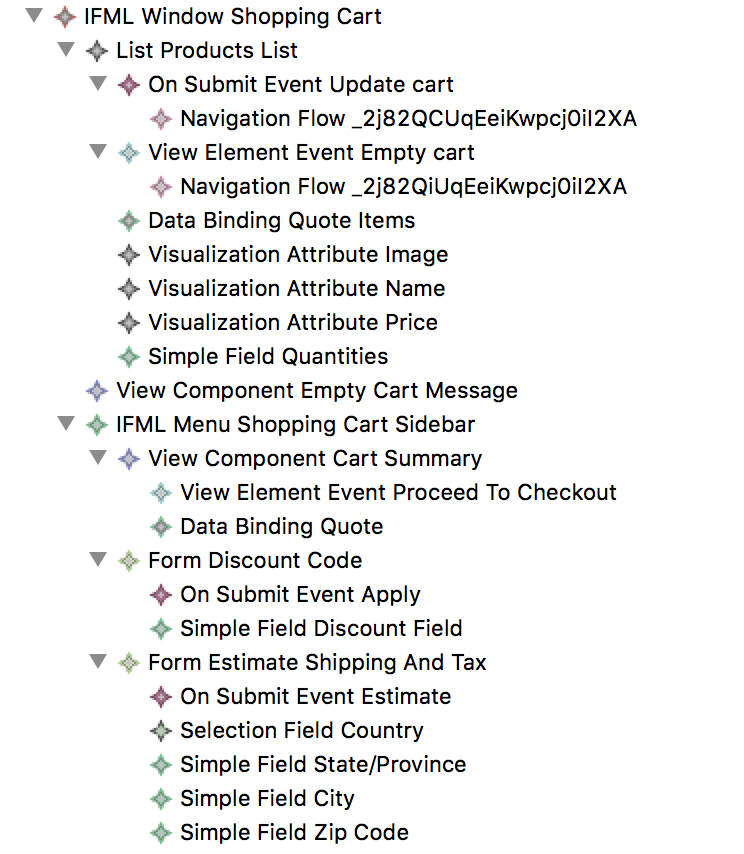
\includegraphics[height=10cm]{images/diagrams/before/ifml-hierarchy-shoppingcart.png}
  \caption{Interaction Flow Shopping Cart Model eCore representation}
  \label{fig:ifml-before-hierarchy-shoppingcart}
\end{figure}
\vspace{0.5cm}

\subsubsection{Shared Elements and Interactions}

As per previously mentioned, shared sections of the platform such as the Header and the Footer have been modeled as \textit{IFMLWindow} nodes reachable from any other area of the website, thus their \textit{Landmark} attribute set to true.
In more detail, the Header section contains a Navigation Menu in the form of a \textit{List View Component} with a children \textit{DataBinding} component correlated to the Category domain model and a simple \textit{Form View Component} for the search mechanism. When the user performs a search submitting a keyword the \textit{SearchKeyword} is triggered and the Search Keyword, based on the parameters held in the associated \textit{ParameterBinding} element, \textit{IFMLAction} is executed.  The resulting Search Results page, which presents a sidebar for filtering and a list of items matching the search, is another \textit{IFMLWindow} which structure resembles the "Product List Mode" for a Category Page described earlier (Figure \ref{fig:ifml-before-header-search}).

\vspace{0.5cm}
\begin{figure}[H]
  \centering
    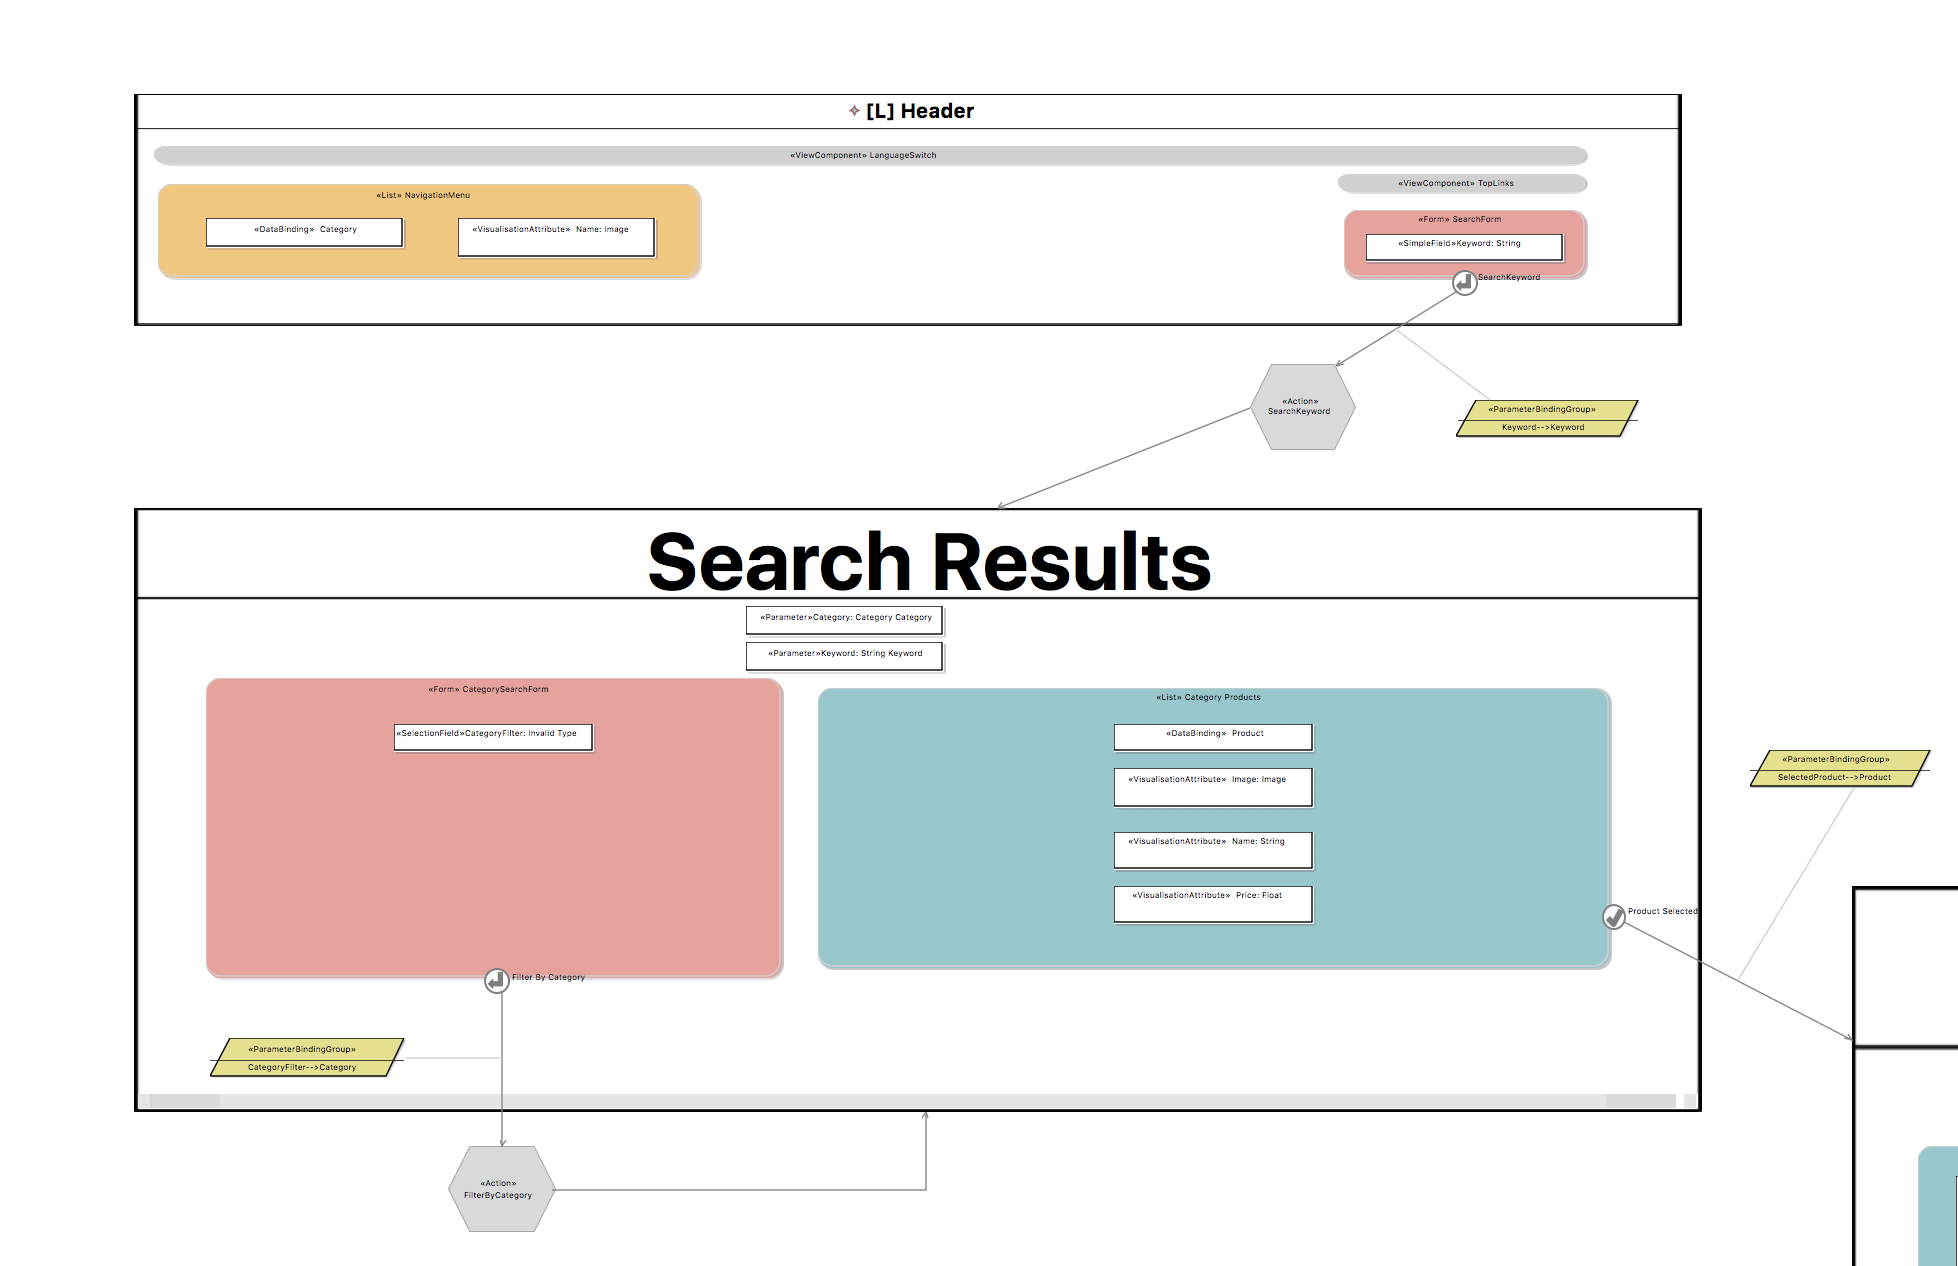
\includegraphics[height=10cm]{images/diagrams/before/ifml-header-search.png}
  \caption{Header and Search sections IFML Diagrams}
  \label{fig:ifml-before-header-search}
\end{figure}
\vspace{0.5cm}

The Footer \textit{IFMLWindow} model is quite straightforward, it retains the information about the footer links presented on the bottom of all the pages of the website in the form of a simple \textit{ViewComponent} and a Newsletter subscription \textit{Form View Component} reacting to SubscribeNewsletter submit \textit{Events}. Like for the header case we just described, the email passed as an argument from the \textit{Event} is carried to the \textit{IFMLAction} which, in this specific case, performs the actual Customer subscription and redirects to the current page.(Figure \ref{fig:ifml-before-footer}).

\vspace{0.5cm}
\begin{figure}[H]
  \centering
    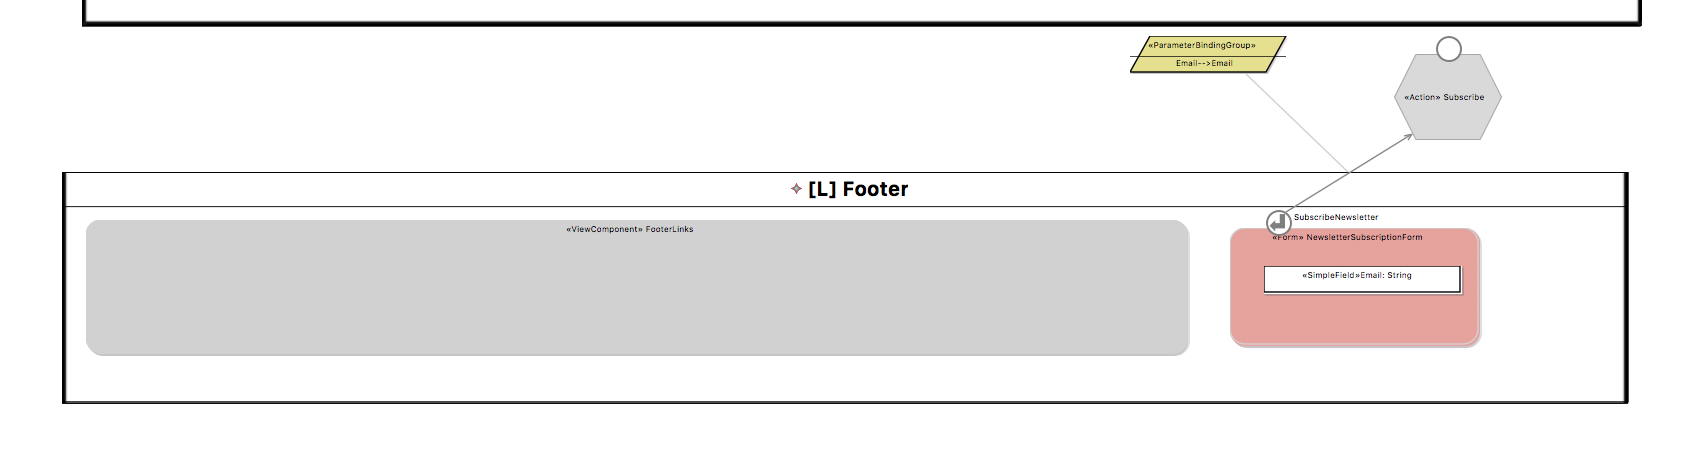
\includegraphics[width=12cm]{images/diagrams/before/ifml-footer.png}
  \caption{Footer section IFML Diagram}
  \label{fig:ifml-before-footer}
\end{figure}
\vspace{0.5cm}

We conclude this chapter with a snippet of the Header \textit{IFMLWindow} element code coming from the \textit{IFMLModel} and an excerpt of the eCore diagram for the areas of the website we described in this subsection (Figure \ref{fig:ifml-before-hierarchy-headersearchfooter}).

\vspace{0.5cm}
\lstset{language=XML}
\begin{lstlisting} 
  <interactionFlowModelElements xsi:type="ext:IFMLWindow" id="_LvuL0BPREei3TrqMA9Bdvw" name="Header" isLandmark="true">
  <viewElements xsi:type="ext:List" id="_v0p5YA9BEeiZ14TmPBeBNA" name="NavigationMenu">
    <viewComponentParts xsi:type="core:DataBinding" id="__mcXIA9BEeiZ14TmPBeBNA" name="Category"/>
    <viewComponentParts xsi:type="core:VisualizationAttribute" id="_Kbzt3xIZEeijSslFDgCgZA" name="Name" featureConcept="//@domainModel/@domainElements.5"/>
  </viewElements>
  <viewElements xsi:type="ext:Form" id="_YWvrMA9GEeiZ14TmPBeBNA" name="SearchForm">
    <viewElementEvents xsi:type="ext:OnSubmitEvent" id="_ULm7WRIWEeijSslFDgCgZA" name="SearchKeyword" viewElement="//@interactionFlowModel/@interactionFlowModelElements.4/@viewElements.1">
      <outInteractionFlows xsi:type="core:NavigationFlow" id="_Y6uV1xIWEeijSslFDgCgZA" targetInteractionFlowElement="//@interactionFlowModel/@interactionFlowModelElements.3">
        <parameterBindingGroup id="_yCY84hPOEei3TrqMA9Bdvw">
          <parameterBindings id="_y5vbohPOEei3TrqMA9Bdvw" sourceParameter="//@interactionFlowModel/@interactionFlowModelElements.4/@viewElements.1/@viewComponentParts.0" targetParameter="//@interactionFlowModel/@interactionFlowModelElements.3/@parameters.0"/>
        </parameterBindingGroup>
      </outInteractionFlows>
    </viewElementEvents>
    <viewComponentParts xsi:type="ext:SimpleField" id="_lWoCAA9GEeiZ14TmPBeBNA" name="Keyword" direction="out">
      <type xsi:type="uml:PrimitiveType" href="model.uml#_VK2hkJ6QEeGdnpRmAZh-dQ"/>
    </viewComponentParts>
  </viewElements>
  <viewElements xsi:type="core:ViewComponent" id="_aQFfjQ9TEeiZ14TmPBeBNA" name="TopLinks"/>
  <viewElements xsi:type="core:ViewComponent" id="_ezXdfQ9TEeiZ14TmPBeBNA" name="LanguageSwitch"/>
</interactionFlowModelElements>
\end{lstlisting}
\vspace{0.5cm}


\vspace{0.5cm}
\begin{figure}[H]
  \centering
    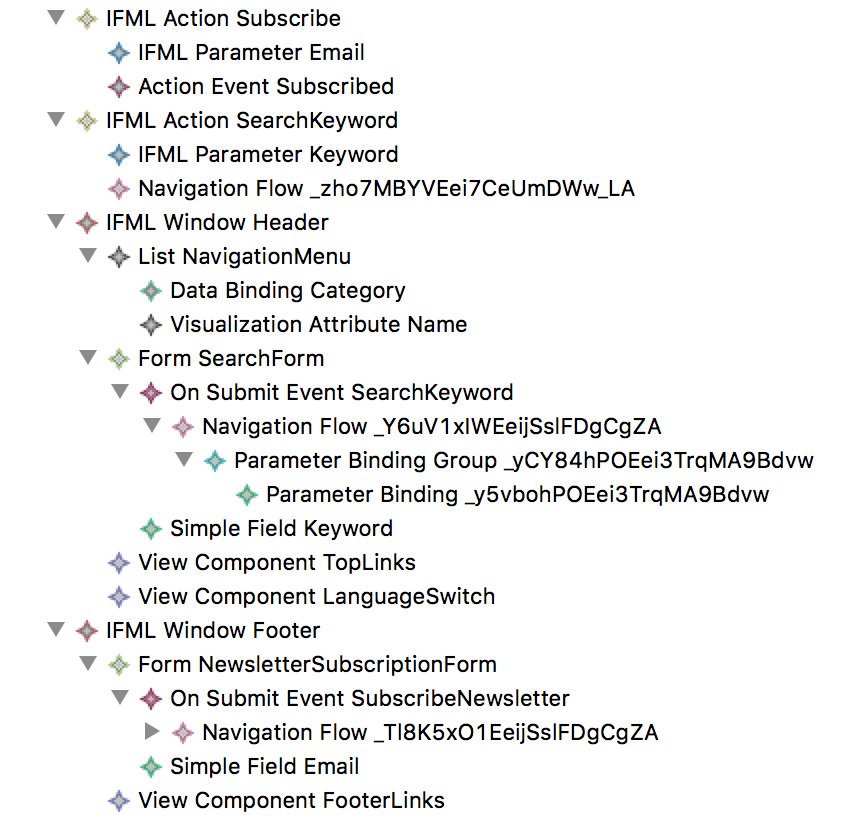
\includegraphics[height=10cm]{images/diagrams/before/ifml-hierarchy-headersearchfooter.png}
  \caption{Interaction Flow eCore representation for the shared elements}
  \label{fig:ifml-before-hierarchy-headersearchfooter}
\end{figure}
\vspace{0.5cm}

